% thesis.tex -- a sample thesis document in dalthesis.cls package
% This is a relatively simple thesis example which can be used to
% start writing your thesis.
\documentclass[12pt, glossary]{dalthesis}

% These packages are not mandatory but they are generally recommended.
% The package graphicx is the common package used to include images in
% the document, usually as a part of a figure:
\usepackage{graphicx}
% The package hyperref is needed to easily navigate through the thesis
% PDF file by making citations clickable, elements of the table of
% contents, URLs, etc.  Including it just by default like this:
%\usepackage{hyperref}
% creates red-bordered boxes around clickable items, which although
% helpful to notice clickable areas do not look nice.  A way to hide
% those boxes, but change colour of clickable text is as follows:
\usepackage[hidelinks]{hyperref}
\hypersetup{
  colorlinks=true,
  linkcolor=blue,
  citecolor=black,
  filecolor=magenta,
  urlcolor=blue, }

\usepackage{graphicx} % Required for inserting images
\usepackage{supertabular,booktabs}
\usepackage{url}
\usepackage{hyperref} 
% \usepackage{mathabx}
\usepackage{etc}
\usepackage{mdframed}
\usepackage{tikz}
\usepackage{pgfplots} 
\usepackage{color,soul}
\usepackage{listings}
\usepackage{balance}
\usepackage{array}
\usepackage[table]{xcolor}
\usepackage{caption}

\usepackage{algorithm}
\usepackage{algpseudocode}
\usepackage{amsmath}
\usepackage{multirow, multicol}
\usepackage{wrapfig}
\usepackage{makecell}
\usepackage{tabularx}
\usepackage{subcaption}
\usepackage{etoolbox}
\usepackage{epigraph}

\usepackage{minted}
\usepackage{listings}
\usepackage{pdfpages}

\usepackage[a-1b]{pdfx}

\lstloadlanguages{Ruby}
\lstloadlanguages{Java}
\lstset{%
basicstyle=\ttfamily\color{black},
commentstyle = \ttfamily\color{red},
keywordstyle=\ttfamily\color{blue},
stringstyle=\color{orange}}




\newcommand{\repositoriesAnalyzed}{x}
\newcommand{\bn}{\textit{Bayes Network}}
\newcommand{\dt}{\textit{Decision Tree}}
\newcommand{\nb}{\textit{Naive Bayes}}
\newcommand{\svm}{\textit{Support Vector Machine}}
\newcommand{\lda}{\textit{Linear Discriminant Analysis}}
\newcommand{\ibk}{\textit{Instance-Based Learner}}
\newcommand{\lkm}{\textit{Lazy K-means}}
\newcommand{\mlp}{\textit{Multilayer Perceptron}}
\newcommand{\lr}{\textit{Linear Regression}}
\newcommand{\logr}{\textit{Logistic Regression}}
\newcommand{\poly}{\textit{Polynomial Regression}}
\newcommand{\rf}{\textit{Random Forest}}
\newcommand{\lb}{\textit{Logit Boost}}
\newcommand{\ada}{\textit{AdaBoost}}
\newcommand{\bg}{\textit{Bagging}}
\newcommand{\knn}{\textit{K Nearest Neighbors}}
\newcommand{\ENDE}{\textit{Encoder-Decoder}}
\newcommand{\latentda}{\textit{Latent Dirichlet Allocation}}

\newcommand{\exm}{\textit{extract method}}
\newcommand{\Exm}{\textit{Extract method}}
\newcommand{\mm}{\textit{move method}}
% \newcommand{\GCB}{\textit{GraphCodeBERT}}
\newcommand{\GCB}{\textsc{g}raph\textsc{c}ode\textsc{bert}}

\newcommand{\RNN}{{\sc rnn}}
\newcommand{\CNN}{{\sc cnn}}
\newcommand{\LSTM}{{\sc lstm}}
\newcommand{\GRU}{{\sc gru}}
\newcommand{\SVM}{{\sc svm}}
\newcommand{\TFIDF}{{\sc tf-idf}}
\newcommand{\rtnn}{\textit{Reverse neural network}}
\newcommand{\DNN}{{\sc dnn}}
\newcommand{\ANN}{{\sc ann}}
\newcommand{\NMT}{{\sc nmt}}
\newcommand{\MLP}{{\sc mlp}} %multi-layer perceptron
\newcommand{\NB}{{\sc nb}} 
\newcommand{\RF}{{\sc rf}} 
\newcommand{\LR}{{\sc lr}} 
\newcommand{\DT}{{\sc dt}} %decision tree
\newcommand{\NLP}{{\sc nlp}}
\newcommand{\KNN}{{\sc knn}}
\newcommand{\BN}{{\sc bn}}
\newcommand{\GNN}{{\sc gnn}}
\newcommand{\dl}{{\sc dl}}
% \newcommand{\llm}{{\sc llm}}

% \newcommand{\exm}{\textit{extract method}}
% \newcommand{\Exm}{\textit{Extract method}}
\newcommand{\llm}{large language model}
\newcommand{\llmsc}{\textsc{llm}}
\newcommand{\Llm}{Large language model}
\newcommand{\LLM}{Large Language Model}
\newcommand{\PPO}{Proximal Policy Optimization}
\newcommand{\ppo}{\textsc{ppo}}
\newcommand{\plbart}{\textsc{plbart}}
\newcommand{\codetf}{\textsc{c}ode-\textsc{t}5}
\newcommand{\codegpt}{\textsc{c}ode\textsc{gpt}-adapt}
\newcommand{\codegen}{\textsc{c}ode\textsc{g}en}
\newcommand{\abst}{\textsc{ast}}
\newcommand{\sft}{\textsc{sft}}


\newcommand*\circled[1]{\tikz[baseline=(char.base)]{
            \node[shape=circle,draw,fill=black!75,color=black!75,text=white,inner sep=1pt] (char) {#1};}}


% \epigraphsize{\small}% Default
\setlength\epigraphwidth{0.5\textwidth}
\setlength\epigraphrule{0pt}


\makeatletter
\patchcmd{\epigraph}{\@epitext{#1}}{\itshape\@epitext{#1}}{}{}
\makeatother


\begin{document}

\title{Semantic and Execution-Aware Extract Method Refactoring via Self-Supervised Learning and Reinforcement Learning-Based Model Alignment}
\author{Indranil Palit}
\supervisor{Dr. Tushar Sharma}
% The following degrees are included in the current dalthesis.cls
% class file:
\mcs  % options are \mcs, \macs, \mec, \mhi, \phd, and \bcshon

% If you degree is not included, you can set several options manually.
% The following example shows the parameters for the \mcs degree.
% However, if you need to set these parameters manually, please check
% the correct names with the Faculty of Graduate Studies, and let the
% maintainer of this class file know (Vlado Keselj, vlado@cs.dal.ca).
% MCS Example:

\degree{Master of Computer Science}
\degreeinitial{M.C.Sc.}
\faculty{Computer Science}
\dept{Faculty of Computer Science}

% Month and Year of Defence
\defencemonth{December}\defenceyear{2024}

\dedicate{To my beloved parents, my younger brother, and my past self, who thought, \textit{``Yeah, this sounds like a great idea!"}}

% This sample thesis contains no tables nor figures, so there is no
% need to include lists of tables and figures in the front matter:
% \nolistoftables
% \nolistoffigures



\frontmatter

\begin{abstract}
% \begin{abstract}
% \begin{abstract}
% \include{abstract}
Software code refactoring is essential for maintaining and improving code quality, yet it remains challenging for practitioners. While modern tools help identify where code needs refactoring, the current implementation techniques often miss meaningful refactoring opportunities. This accumulates technical debt over time, making software increasingly difficult to maintain and evolve. This thesis presents an automated hybrid approach to identify refactoring candidates and generate refactored code leveraging language models and reinforcement learning.

The first major contribution of the thesis addresses the shortcomings of automatic refactoring candidate identification by training machine learning classifiers with rich code semantics. Unlike traditional approaches that rely on metrics and commit messages, we've developed a self-supervised learning approach to identify negative samples utilizing state-of-the-art GraphCodeBERT embeddings. This approach achieves a $30$\% improvement in F1 score compared to existing metric-based techniques to identify extract method refactoring candidates automatically. 



Our second contribution introduces a novel approach to automated code refactoring using reinforcement learning, with a specific focus on extract method refactoring. While recent advances in large language models have shown promise for code transformation, traditional supervised learning approaches often fail to produce reliable results. These models typically struggle with maintaining code integrity because they treat code generation similar to text generation, overlooking crucial aspects like compilability and functional correctness. To address this limitation, we develop a method that fine-tunes state-of-the-art pre-trained code language models (e.g., CodeT5) with Proximal Policy Optimization (PPO), creating a code-aware transformation framework. Our approach uses carefully designed reward signals based on successful compilation and adherence to established refactoring guidelines, moving beyond simple text-based metrics. When tested against conventional supervised learning methods, our system demonstrates significant improvements in quality and quantity. 

\newpage
Together, these advances mark a significant step toward automated, reliable code refactoring that can effectively reduce software practitioner's burden while maintaining high software quality standards. The success of our approach demonstrates how modern machine learning and deep learning techniques when carefully adapted to understand code semantics, can transform traditional software engineering practices.


\end{abstract}
Software code refactoring is essential for maintaining and improving code quality, yet it remains challenging for practitioners. While modern tools help identify where code needs refactoring, the current implementation techniques often miss meaningful refactoring opportunities. This accumulates technical debt over time, making software increasingly difficult to maintain and evolve. This thesis presents an automated hybrid approach to identify refactoring candidates and generate refactored code leveraging language models and reinforcement learning.

The first major contribution of the thesis addresses the shortcomings of automatic refactoring candidate identification by training machine learning classifiers with rich code semantics. Unlike traditional approaches that rely on metrics and commit messages, we've developed a self-supervised learning approach to identify negative samples utilizing state-of-the-art GraphCodeBERT embeddings. This approach achieves a $30$\% improvement in F1 score compared to existing metric-based techniques to identify extract method refactoring candidates automatically. 



Our second contribution introduces a novel approach to automated code refactoring using reinforcement learning, with a specific focus on extract method refactoring. While recent advances in large language models have shown promise for code transformation, traditional supervised learning approaches often fail to produce reliable results. These models typically struggle with maintaining code integrity because they treat code generation similar to text generation, overlooking crucial aspects like compilability and functional correctness. To address this limitation, we develop a method that fine-tunes state-of-the-art pre-trained code language models (e.g., CodeT5) with Proximal Policy Optimization (PPO), creating a code-aware transformation framework. Our approach uses carefully designed reward signals based on successful compilation and adherence to established refactoring guidelines, moving beyond simple text-based metrics. When tested against conventional supervised learning methods, our system demonstrates significant improvements in quality and quantity. 

\newpage
Together, these advances mark a significant step toward automated, reliable code refactoring that can effectively reduce software practitioner's burden while maintaining high software quality standards. The success of our approach demonstrates how modern machine learning and deep learning techniques when carefully adapted to understand code semantics, can transform traditional software engineering practices.


\end{abstract}
Software code refactoring is essential for maintaining and improving code quality, yet it remains challenging for practitioners. While modern tools help identify where code needs refactoring, the current implementation techniques often miss meaningful refactoring opportunities. This accumulates technical debt over time, making software increasingly difficult to maintain and evolve. This thesis presents an automated hybrid approach to identify refactoring candidates and generate refactored code leveraging language models and reinforcement learning.

The first major contribution of the thesis addresses the shortcomings of automatic refactoring candidate identification by training machine learning classifiers with rich code semantics. Unlike traditional approaches that rely on metrics and commit messages, we've developed a self-supervised learning approach to identify negative samples utilizing state-of-the-art GraphCodeBERT embeddings. This approach achieves a $30$\% improvement in F1 score compared to existing metric-based techniques to identify extract method refactoring candidates automatically. 



Our second contribution introduces a novel approach to automated code refactoring using reinforcement learning, with a specific focus on extract method refactoring. While recent advances in large language models have shown promise for code transformation, traditional supervised learning approaches often fail to produce reliable results. These models typically struggle with maintaining code integrity because they treat code generation similar to text generation, overlooking crucial aspects like compilability and functional correctness. To address this limitation, we develop a method that fine-tunes state-of-the-art pre-trained code language models (e.g., CodeT5) with Proximal Policy Optimization (PPO), creating a code-aware transformation framework. Our approach uses carefully designed reward signals based on successful compilation and adherence to established refactoring guidelines, moving beyond simple text-based metrics. When tested against conventional supervised learning methods, our system demonstrates significant improvements in quality and quantity. 

\newpage
Together, these advances mark a significant step toward automated, reliable code refactoring that can effectively reduce software practitioner's burden while maintaining high software quality standards. The success of our approach demonstrates how modern machine learning and deep learning techniques when carefully adapted to understand code semantics, can transform traditional software engineering practices.


\end{abstract}


\begin{acknowledgements}
% Thanks to all the little people who make me look tall.
\noindent

Firstly, I can't thank Dr. Tushar Sharma enough. He's been an incredible supervisor since before I even joined Dalhousie. The trust he placed in me was amazing! Beyond research guidance, he helped with teaching opportunities and external projects. What makes him special is how approachable he is - whether it's academic or personal issues, his door was always open. While I wasn't always a perfect student and made mistakes along the way, he helped me learn and grow from each experience. His endless encouragement, thoughtful guidance, and understanding nature made this thesis possible. Tushar, you're the best mentor I could've asked for - thank you for everything!

To the members of our Software Maintenance and Analytics Research Team (SMART) lab - Mootez Saad, Saurabhsingh Rajput and Gautam Shetty, I consider myself to be extremely fortunate to have met you all and got the opportunity to work alongside such great minds. I am also grateful for all the interactive lab meetings we had, from brainstorming research ideas to dreaming up (hilariously failed) startup plans. Those late night discussions about everything under the sun - football, politics, food recipes, and those endless jokes, are memories I'll always cherish. I would like to specially thank my exceptionally talented and hard working friend and peer, Mootez, for time and again helping me with my research providing his insightful feedback and inputs. These suggestions had a significant impact in polishing my work. Working with him was truly inspirational. I would also like to thank the previous members and interns of our lab. It is an honor to become an alumni of this lab.

To Saurabh and Gautam, this section doesn't have sufficient space to accommodate everything that they have done for me. We three have become brothers since day one. Every memory in Halifax involves these two - from last minute assignment rushes and technical discussions to exploring the city together, watching football matches, and impromptu trips. Saurabh's laid-back attitude and reassuring presence with deep technical knowledge helped me navigate through challenging times. Gautam's wisdom and thoughtful insights, both on and off work discussions have been invaluable. I am also indebted to Gautam for his valuable contribution as an author in my first research paper.

I am deeply thankful to all the members of the Intelligent Automation in Software EngineeRing (RAISE) lab - Mehil B Shah, Asif Samir, Usmi Mukherjee, Sigma Jahan and Riasat Mahbub. I would like to acknowledge and appreciate my very good friends Usmi, Mehil and Sigma for supporting me and cheering me both professionally and personally. Mehil is very vocal and I admire his innocence and authentic presence. Sigma is a multi-tasker and I really think she has invisible octopus hands. Finally, I would like to thank Usmi for being there as a friend and a strong support system throughout the journey. She is one of the best people I ever met. Also, she is the only friend from my hometown, Kolkata. Celebrating Durga Puja as \textit{probashi bangalis} (expatriate bengalis) will always be a great experience.

I would like to extend my sincere gratitude towards Dalhousie University and the Faculty of Computer Science for providing me with this splendid learning opportunity. I would like to thank Dr. Michael McAllister for promptly resolving a major administrative issue I was facing. I would also like to thank the department for awarding me with graduate bursaries twice. I am very fortunate to have received funding support from \texttt{NRC IRAP}, \texttt{Lab2Market} and \texttt{Mitacs Accelerate}. The internships and projects enabled by this funding provided valuable opportunities to apply my research in practical, real-world settings. The defense

This graduate journey would not have been possible without the constant support and encouragement from my incredible parents, brother and other close family members, who have stood by me every step of the way. I am deeply grateful for their belief in me and the strength they have given me throughout this journey. I would also like to take a moment to thank all my friends back home, especially Jessica Banik and Swagnik Banerjee, whose friendship and support have been invaluable during this transformative phase of my life. 

Lastly, I sincerely thank everyone who supported me throughout this research journey. Their encouragement, advice, and assistance have been invaluable, and I am truly grateful.
\end{acknowledgements}

\mainmatter


\chapter{Introduction}
\epigraph{Any fool can write code that a computer can understand. Good programmers write code that humans can understand.}{--- \textup{Martin Fowler}}



This opening chapter frames our research presented in this thesis, by establishing its context, identifying the key challenges in software refactoring, describing our proposed methodology, and highlighting the main contributions of this work.

\section{Code quality}

Software quality is about more than just ticking boxes on a requirements list. While we can measure it by how well the code matches technical specifications, the real test is whether it actually helps people do what they need to do. At its core, quality software should both work as designed and make users' lives easier ~\cite{spinellis2006code}. Poor quality choices tend to have lasting consequences, often creating technical debt that impacts projects long after release~\cite{seaman2011measuring}. 

In software engineering, quality encompasses two fundamental dimensions: functional and structural~\cite{balci1998verification}. Functional quality measures how effectively software meets its specified design requirements and fulfills its intended purpose, essentially determining if we built the right software. Structural quality, on the other hand, focuses on the non-functional attributes such as maintainability, reliability, and robustness, determining if we built the software right~\cite{madler2021applying}. Together, these dimensions ensure that software not only provides the right features but also performs efficiently and remains sustainable throughout its lifecycle.

Maintainability encompasses key attributes such as modularity, understandability, and testability that determine how easily software can be modified and managed. Studies have shown that poor maintainability practices lead to $40$-$70$\% of the total software lifecycle costs~\cite{seacord2003modernizing}. 
% Rather than manifesting as major code issues, poor maintainability typically stems from numerous small deviations from best practices, leading to what is known as technical debt --- the long-term costs resulting from maintainability issues.

Code maintainability problems often reveal themselves through what software practitioners call ``code smells" - patterns that signal potential design flaws~\cite{Fowler1999Refactoring}. Just as unpleasant odors can signal health hazards in our environment, code smells warn of deeper implementation~\cite{Fowler1999Refactoring}, design~\cite{suryanarayana2014refactoring} or architectural~\cite{garcia2009identifying} issues. Common examples include duplicated code blocks, overly complex methods, and tightly coupled components. While these patterns don't necessarily indicate immediate bugs, they make the codebase increasingly difficult to understand, maintain, and modify. Over time, these issues compound, leading to higher development costs and reduced team productivity, particularly when teams need to add new features or fix existing problems.

\section{Problem statement}

% \begin{minipage}[]{\columnwidth}
%     \footnotesize
%     \begin{minipage}[]{0.60\columnwidth}
%         \paragraph{Example Code}
%         \label{lst:branching_code}
%         \inputminted[breaklines=True]{java}{chapters/example_codes/cs1.java}
%         % \paragraph{X86 Assembly}
%         % \inputminted{asm}{code/branching_other_function.s}
%     \end{minipage}
%     \hfill
%     % \begin{minipage}[]{0.35\linewidth}
%     %     \paragraph{Branchless Code}
%     %     \label{lst:branchless_code}
%     %     \inputminted{c++}{code/Minimax_perf.cpp}
%     %     \vspace{1.1cm}
%     %     \paragraph{X86 Assembly}
%     %     \inputminted{asm}{code/branchless_other_function.s}
%     %     \vspace{3.6cm}
%     % \end{minipage}
% \end{minipage}



One of the code smells, the \textit{long method} smell, characterized by methods that are excessively long and complex, is particularly prevalent in Object-Oriented Programming (OOP)~\cite{fowler2018refactoring, Sharma2018}. Recent systematic reviews and empirical studies have consistently ranked the long method smell among the top five most frequently occurring and problematic code smells~\cite{agnihotri2020systematic, lacerda2020code}.

The primary remedy for addressing the long method smell is \textit{Extract Method} refactoring~\cite{Fowler1999Refactoring}. This technique involves identifying cohesive blocks of statements within a long method and extracting them into a separate, well-named method.

However, the current practice of \exm{} refactoring presents several challenges:
\begin{itemize}
    \item {Manual Identification}: Developers must first identify methods that require refactoring and then locate specific code blocks suitable for extraction, a process that becomes increasingly complex and time-consuming as codebase size grows.
    \item {Error-Prone Implementation}: The manual extraction process can inadvertently introduce new bugs or even create new code smells, particularly when dealing with complex method dependencies and variable scoping.
    \item {Automated Tool Support}: The existing tools and IDE plugins that assist software practitioners to perform extract method refactoring are not fully automated. The user has to specify which block of code needs needs the refactoring and then the tool simply extracts that block.
\end{itemize}

While some approaches have been proposed to address the long method smell~\cite{maruyama2001automated, tsantalis2011identification, charalampidou2016identifying}, these solutions are not fully automated and still require significant manual intervention to complete the refactoring process. The lack of a comprehensive, automated solution for both identifying and executing \exm{} refactoring opportunities represents a significant gap in modern software maintenance tools and practices.

\section{Motivating example}
To illustrate the challenges and importance of automated extract method refactoring, consider the following real-world code example from Netflix's {Eureka} project at commit {756bcd9}~\footnote{\href{https://github.com/Netflix/eureka/blob/756bcd9fd308647c7b388543da9a3a6e034ee3f5/eureka-client/src/main/java/com/netflix/discovery/DiscoveryClient.java\#L865}{Netflix Eureka DiscoveryClient.java}}, a service registry for microservices architectures:

\begin{listing}[H]
    \footnotesize
    \centering
    \caption{Extract Method Refactoring Candidate}
    \label{lst:branching_code}
    \inputminted[breaklines=true, breakafter=-, breaksymbolleft={},
    linenos=true, bgcolor=gray!10, highlightlines={16-25}]{java}{chapters/example_codes/motex.java}
\end{listing}

This method combines status retrieval and event publishing logic with complex control flow and exception handling.
The refactored version separates these concerns more effectively:

% \begin{minipage}[]{\columnwidth}
%     \footnotesize
%     \begin{minipage}[]{\columnwidth}
%         \caption {Code after Extract Method Refactoring}
%         % \paragraph{Code after Extract Method Refactoring}
%         \label{lst:branching_code}
%         \inputminted[breaklines=true, breakafter=-, breaksymbolleft={},
%         linenos=true, bgcolor=gray!10, highlightlines={6,13-22}]{java}{chapters/example_codes/motex2.java}
%     \end{minipage}
% \end{minipage}

\begin{listing}[H]
    \footnotesize
    \centering
    \caption{Code after Extract Method Refactoring}
    \label{lst:branching_code}
    \inputminted[breaklines=true, breakafter=-, breaksymbolleft={},
    linenos=true, bgcolor=gray!10, highlightlines={15,19-25}]{java}{chapters/example_codes/motex2.java}
\end{listing}

The refactoring improves the code by separating concerns, simplifying error handling, and enhancing testability. However, identifying such opportunities in large codebases requires careful analysis of context, variable scope, and behavior preservation. This example demonstrates the need for an automated approach to detect and perform such refactorings consistently across large-scale systems.

\section{Proposed Solution and Contribution}

\subsection{Proposed solution}
We present a novel, fully automated two-phased approach to address the challenges of extract method refactoring.

\textbf{Phase 1---Refactoring Candidate Identification:}\
We develop an innovative approach to identify potential candidates for \exm{} refactoring by generating source code embeddings and advanced machine learning classifiers. This phase focuses on identifying candidates suitable for \exm{} refactoring.

\textbf{Phase 2---Automated Refactoring Generation:}\
We implement an intelligent refactoring system using Large Language Models (\llmsc{}), enhanced through fine-tuning and Reinforcement Learning (\rl{}) optimization. This approach focuses on to generate refactored code that maintains both syntactic correctness and semantic equivalence with the original implementation.

\subsection{Key contributions}
This thesis makes the following contributions to the field of automated software refactoring:

\begin{itemize}
\item \textbf{Novel Sample Identification Framework:} We introduce a systematic mechanism for identifying and classifying positive and negative samples for \exm{} refactoring, addressing a fundamental gap in existing approaches.

\item \textbf{Comprehensive Benchmark Dataset:} We develop a large-scale dataset comprising $55,430$ labeled samples (both positive and negative), establishing a robust benchmark for evaluating automated refactoring candidate identification approaches.

\item \textbf{Advanced Code Representation:} We propose an Autoencoder-based approach that leverages \GCB{} for extracting latent features, enabling more effective method representation for binary classification tasks.

\item \textbf{Supervised Fine-tuning Framework:} We develop and evaluate supervised fine-tuned models specifically designed for automatic \exm{} refactoring, eliminating the need for manual code block selection and addressing key limitations of existing approaches.

\item \textbf{Hybrid Learning Architecture:} We present a novel hybrid approach that combines supervised fine-tuning with reinforcement learning optimization, specifically engineered for extract method refactoring. The effectiveness of this approach is validated through both quantitative metrics and qualitative analysis.

\item \textbf{Open-source Tool and Dataset:} We contribute a comprehensive tool for analyzing Java repositories on GitHub to generate extract method refactoring datasets with detailed metadata. Both the tool and the resulting dataset are made publicly available in Appendix~\ref{appendix} to facilitate replication studies and future research extensions.

\end{itemize}

\section{Related Publication}

Parts of this research work has been either accepted at or submitted to the following conferences.

\begin{itemize}
    \item Palit, Indranil, Gautam Shetty, Hera Arif, and Tushar Sharma.``Automatic refactoring candidate identification leveraging effective code representation." In 2023 IEEE International Conference on Software Maintenance and Evolution (ICSME), pp. 369-374. IEEE, 2023.
    
    \item Palit, Indranil and Tushar Sharma.``Reinforcement Learning vs Supervised Learning: A tug of war to generate refactored code accurately" Proceedings of the ACM on Software Engineering 1, no. FSE (2025) (\textit{submitted})
\end{itemize}

\vspace{\fill}
\section{Outline of the Thesis}

This thesis presents an end-to-end solution for automating \exm{} refactoring through two interconnected studies, organized into five chapters:

\begin{itemize}
    \item \textbf{Chapter 2} Introduces fundamental concepts in software refactoring, code embeddings, transformer architectures, and reinforcement learning that form the foundation for our technical approaches.

    \item \textbf{Chapter 3} Presents our first contribution: an innovative approach using code embeddings and machine learning to automatically identify potential \exm{} refactoring candidates.

    \item \textbf{Chapter 4} Describes our second contribution: a novel reinforcement learning-based framework that automatically transforms identified candidates into properly refactored methods.

    \item \textbf{Chapter 5} Synthesizes our findings and outlines promising directions for future research in automated code refactoring.
\end{itemize}


\chapter{Background and Related work}

\epigraph{Research is to see what everybody else has seen, and think what nobody has thought.}{--- \textup{Dr. Albert Szent-Gyorgyi}}

This chapter has two main sections. The first section provides the background concepts needed to understand our research. The second section reviews existing research in this field, examining prior work that shapes the basis of our study.

\section{Context}

\subsection{Extract method refactoring}
Extract Method refactoring, first formalized by Fowler \cite{Fowler1999Refactoring}, is a fundamental technique for improving code maintainability by decomposing large methods into smaller, more focused units. This transformation involves identifying cohesive code fragments and extracting them into new methods while preserving program behavior \cite{murphy2011we}. Recent studies by Silva~\etal{} \cite{silva2016we} and Tsantalis~\etal{} \cite{Tsantalis2018Accurate} have shown that Extract Method is among the most frequently applied refactorings in practice, accounting for approximately 15-25\% of all refactoring operations in large-scale systems.

The primary motivation for Extract Method refactoring is to address the``Long Method" code smell, where methods become long, complex or incohesive, violating the single responsibility principle \cite{martin2009clean}. The process involves identifying a coherent fragment of code, extracting it into a new method with an appropriate name, and replacing the original fragment with a call to the newly created method. This transformation must preserve program semantics while managing variable scope, parameter passing, and return values \cite{kim2012field}. Studies by Murphy-Hill et al. \cite{murphy2011we} have shown that while developers frequently perform this refactoring manually, automated tool support remains challenging due to the complexity of ensuring behavioral preservation and identifying optimal extraction points.

\subsection{Embeddings}

Code embeddings are dense vector representations that capture semantic properties of source code in a continuous space. Alon~\etal{} \cite{Alon2019Code2vec} introduced Code2Vec, demonstrating how path-based attention over abstract syntax trees can create meaningful code representations. This was further advanced by Feng~\etal{}. \cite{feng2020codebert} with CodeBERT, which combines both structural and textual features of code. These embedding techniques have revolutionized code analysis by enabling deep learning models to better understand and process source code semantics.

Recent advancements in code embeddings have focused on incorporating multiple views of code, such as data flow, control flow, and natural language documentation. Guo et al. \cite{guo2022unixcoder} demonstrated that unified representations combining these different aspects significantly improve performance on some downstream tasks. The effectiveness of these embeddings has been particularly evident in tasks such as code similarity detection, bug localization, and automated program repair \cite{zhou2019devign}. Furthermore, studies by Kanade~\etal{} \cite{kanade2020learning} have shown that pre-training on large code corpora can create embeddings that capture rich semantic relationships between different programming concepts and patterns.

\subsection{Transformers}

The Transformer architecture, introduced by Vaswani~\etal{} \cite{vaswani2017attention}, revolutionized sequence processing through its self-attention mechanism. In the context of code processing, Ahmad~\etal{} \cite{ahmad2021} demonstrated how Transformers can effectively capture long-range dependencies in source code, while Hellendoorn~\etal{} \cite{hellendoorn2019global} showed their effectiveness in modeling code structure through global attention patterns. The architecture's ability to process sequences in parallel while maintaining contextual relationships has made it particularly suitable for code analysis tasks.

The key innovation of Transformers lies in their self-attention mechanism, which allows the model to weigh the importance of different parts of the input sequence dynamically. For code processing, this is particularly valuable as it enables the model to capture relationships between distant parts of the code, such as variable declarations and their uses, or function calls and their definitions \cite{wang2019self}. Recent adaptations of the Transformer architecture for code, such as CodeT5 \cite{wang2021codet5identifierawareunifiedpretrained}, have introduced specialized attention patterns that better align with code structure, including syntax-aware attention and hierarchical representations that respect code's abstract syntax tree structure.

% \subsection{Large Language Models}

\subsection{Supervised fine-funing of large language models}


Supervised fine-tuning is an add-on training for adapting pre-trained large language models (LLMs), such as CodeT5~\cite{wang2021codet5identifierawareunifiedpretrained}, to specialized tasks. 
This adaptation is achieved by training the models on domain-specific datasets, which is particularly important for enhancing their performance in tasks such as extract method refactoring. In this context, we focus on two predominant model architectures: \textit{encoder-decoder} and \textit{decoder-only} models.

Encoder-decoder models consist of two main components. 
The encoder processes the input sequence (\ie{} source code, in our case) to create a context-rich representation, which the decoder then uses to generate the output sequence (refactored code with extracted method, in our case).
This architecture is particularly useful when the input is a code snippet, and the output is the corresponding refactored version. 
The fine-tuning objective for encoder-decoder models aims to maximize the conditional probability of the correct output sequence given an input sequence. 
% During training, inputs are fed into the encoder, and their corresponding target outputs into the decoder. 
A technique called teacher forcing is employed, where the correct output token from the previous time step is fed as input to the next step. 
% \todo{rewrite this using autoregressive characteristic - I am not sure if enc-dec models have autoregressive characteristics. Do you mean the autoregressive characteristics of the decoder?}

Decoder-only models, such as those used in GPT-like architectures~\cite{radford2019language}, operate differently. They generate each token of the output sequence directly, conditioned on all previous tokens and the input sequence, without a separate encoding phase. The training process involves presenting the combined sequence of the input code and the refactored code to the model, typically separated by a special token, \eg{} ~\textsc{[sep]}.

For both architectures, the loss function commonly used is the cross-entropy loss, calculated over the output sequence tokens. This loss function helps the model learn to predict the correct tokens in the output sequence. 


\subsection{Reinforcement learning for sequence generation}

Reinforcement Learning (\rl{}) is a branch of machine learning focused on 
% teaching algorithms to make a series of decisions~\cite{shakya2023reinforcement}.
training agents to take actions in an environment to maximize some notion of cumulative reward often involving a series of decisions~\cite{shakya2023reinforcement}. 
It uses a model known as the Markov Decision Process (MDP)~\cite{puterman2014markov}, which deals with decision-making where each action is determined by steps, and outcomes are influenced by randomness. 
In \rl{}, an agent (\ie{} an autonomous entity that takes action in the given environment)
improves its decisions through trial-and-error interactions with its environment, learning from the rewards it receives based on its actions. The agent's decision-making strategy is known as the \textit{policy}, which determines the next action to take given the current situation or \textit{state}. The \textit{state} represents the current context or input on which the agent bases its decisions.


In the context of language models, \rl{} can be employed as a training mechanism. 
Here, the language model serves as the \textit{policy}, and the current text sequence is the \textit{state}. 
The model generates an action,
the next word or token,
altering the state into a new text sequence. 
The quality of the completed text sequence determines the reward, assessed either by human judgment or a trained reward model based on human preferences.

Formally, MDP can be defined as follows.

\textbf{State Space: }
The state space \(S\) is the set of all possible language representations up to a maximum length \(L\):
\begin{equation}
    S = \{s \mid s \in \mathbb{R}^d \times l, l \leq L\}
\end{equation}
where \(d\) is the dimensionality of the token embeddings and \(l\) is the current sequence length.

% \subsubsection{Markov Decision Process Definition}
\textbf{Action Space: }
The action of the model (actor) is to generate the next token based on the previously generated tokens and the input data. The action space is the vocabulary of the language model, representing all possible tokens:
\begin{equation}
    A = \{1, 2, \ldots, V\}
\end{equation}
where \(V\) is the vocabulary size.

\textbf{State Transition Function: } 
The state transition function \(P\) describes how the environment moves from one state to another given an action. In our sequence generation task, this transition is deterministic:
\begin{equation} \label{eq:state_trans_func}
    P(s_{t+1} \mid s_t, a_t) = 
    \begin{cases} 
    1 & \text{if } s_{t+1} = [s_t; e(a_t)], \\
    0 & \text{otherwise}
    \end{cases}
\end{equation}
where \(e(a_t)\) is the embedding of the chosen token.

\textbf{Policy: }
The policy is represented by a language model that produces a probability distribution over the next token given the current state:
\begin{equation}
    \pi_\theta(a \mid s) = \text{LM}_\theta(a \mid s)
\end{equation}
where \(\text{LM}_\theta\) is the language model with parameters \(\theta\).

\textbf{Value Function: }
The value function estimates the expected cumulative reward from a given state under a particular policy:
\begin{equation}
    V_\phi(s) = \mathbb{E}_{\pi_\theta}\left[\sum_{t=0}^{\infty} \gamma^t R_t \mid S_0 = s\right]
\end{equation}
where \(\phi\) are the parameters of the value head and \(\gamma\) is the discount factor.

\subsubsection{Reward}
In sequence modeling, the reward quantifies the quality or desirability of generated sequences. It measures how well the generated sequence aligns with desired characteristics, such as fluency, coherence, or task-specific objectives.

\subsubsection*{Reward Function}
The reward function \(R\) can be expressed as:
\begin{equation}
    R(s, a) = \lambda_1 r_{\text{task}}(s, a) + \lambda_2 r_{\text{seq}}(s, a)
\end{equation}
where $r_{\text{task}}$ represents task-specific evaluation metrics, $r_{\text{seq}}$ captures sequence quality measures, and $\lambda_1$, $\lambda_2$ are weighting coefficients balancing different reward components..


In the software engineering domain, \rl{} has been used for code completion tasks~\cite{shojaee2023execution, li2024ircoco} and code summarization~\cite{wan2018improving}. They all use actor-critic methods to train the language models for specific downstream tasks. The actor is the policy model, the main language model pre-trained or fine-tuned on code data and the critic is another component that evaluates the output generated by the actor and provides a reward signal. Based on this architecture, we formulate our problem as follows. 


\subsection{Solution framework}

In this second part of this thesis, we focus on aligning a fine-tuned large language model for extract method refactoring generation using Proximal Policy Optimization (\ppo{})~\cite{schulman2017proximal}---a popular actor-critic  reinforcement learning method. 
This alignment process involves several key components: the actor, the critic, rewards, the value function, and KL divergence.

The \textit{actor} in our setting is the language model itself, which generates sequences of code such as extracting methods from code snippets. It takes the current code as input and outputs a refactored version with extracted methods. The \textit{critic} is a separate component that evaluates the quality of the refactoring produced by the actor, providing a score or reward that reflects how well the generated refactoring meets the desired criteria, such as syntactically and semantically accurate refactored code.

A \textit{reward} is a numerical score assigned to each generated refactoring, indicating its quality. Higher rewards are given for refactorings that improve code properties, while lower rewards indicate poor refactoring outcomes, such as introduction of errors. These rewards guide the actor in learning to generate more desirable refactorings over time.

The \textit{value function} estimates the expected reward from a given state or step in the sequence generation process. It predicts how good the current refactoring is, considering future rewards. In practice, the value function is represented by a separate neural network head, called a \textit{value head}, which outputs a scalar value for each input state, estimating the expected cumulative reward, denoted as 
\begin{equation} \label{eq:value_func}
 V(s) = \mathbb{E} \left[ R \mid s \right], where\ R\ is the\ total\ reward
\end{equation}

\textit{Proximal Policy Optimization (\ppo{})} is the algorithm used to train the actor model. \ppo{} optimizes the model's parameters by adjusting its behavior in small, controlled steps, ensuring that changes are not too drastic. This balance between exploration (trying new refactoring strategies) and stability (maintaining effective behaviors) helps the model learn efficiently without losing its learned knowledge.

The \textit{objective function} in PPO aims to maximize the expected reward while ensuring that updates to the policy (the actor's behavior) are not excessively large. The PPO objective can be formulated as:

\[
L^{\text{PPO}}(\theta) = \mathbb{E} \left[ \min \left( r_t(\theta) \hat{A}_t, \, \text{clip}(r_t(\theta), 1 - \epsilon, 1 + \epsilon) \hat{A}_t \right) \right],
\]

where \( \theta \) represents the model parameters, \( r_t(\theta) = \frac{\pi_\theta(a_t \mid s_t)}{\pi_{\theta_{\text{old}}}(a_t \mid s_t)} \) is the ratio of the new policy to the old policy, \( \hat{A}_t \) is the advantage estimate, and \( \epsilon \) is a small constant controlling the clipping range.

%  

The \textit{PPO loss} combines the clipped objective function with the value function loss and an entropy bonus. The complete loss function can be expressed as:

\[
L(\theta) = L^{\text{PPO}}(\theta) - c_1 \cdot \text{Value Loss}(\theta) + c_2 \cdot \text{Entropy Bonus}(\theta),
\]

where the \textit{Value Loss} measures the accuracy of the critic's value estimates, and the \textit{Entropy Bonus} encourages exploration by preventing the actor from becoming overly deterministic.

\textit{KL Divergence} (Kullback-Leibler divergence) measures the difference between the old policy $\pi_{\theta_{old}}$ and the updated policy $\pi_\theta$, ensuring that updates to the policy do not deviate excessively from the original behavior. It is calculated as:

\begin{equation} \label{eq:kl_div}
\text{KL}(\pi_{\theta_{old}} \parallel \pi_{\theta}) = \sum_{x} \pi_{\theta_{old}}(x) \log \left( \frac{\pi_{\theta_{old}}(x)}{\pi_{\theta}(x)} \right),
\end{equation}

where $\pi_{\theta_{old}}(x)$, $\pi_\theta(x)$ represent the probability distributions over the possible code refactoring actions that the model can take at a given step.

In summary, the actor generates refactoring suggestions, and the critic evaluates them using static non differential rewards that provide feedback on their quality. \ppo{} optimizes the model's behavior gradually, guided by the value function, the objective function, and loss components, 
% \doubt{I haven't included the objective and loss components because it was very difficult to explain without complex math equations. Should I do it or remove it since it might be understood from just PPO? \\
% If they are short equation, you can. Otherwise, mention them using words.}, 
while KL divergence ensures that changes remain within reasonable limits. This framework enables the fine-tuning of the language models to produce high-quality code refactorings over time.


\section{Related Work}

\subsection{Refactoring candidate identification using traditional techniques}

Software developers can manually decide \textit{what} to refactor according to their intuition and past experiences~\cite{Al2015Identifying}.
Often, they use automated tools to calculate code quality metrics and code smells to identify refactoring candidates~\cite{Mens2004Survey, Al2015Identifying}. 
Another method to identify refactoring candidates is to define a set of preconditions or compliance rules. If a code did not follow these rules, it was considered a candidate for refactoring. Studies by Bois \etal{}~\cite{Du2004Refactoring} and Kataoka \etal{}~\cite{Kataoka2001Automated} used such compliance rules.

Another technique considers creating clustering algorithms to identify if code needs refactoring. 
Czibula \etal{}~\cite{Czibula2008Hierarchical} and Serban \etal{}~\cite{Serban2007Restructuring}, 
created clusters based on the distance between methods and attributes within and outside of classes to identify numerous refactoring candidates.
Similarly, Bavota \etal{}~\cite{Bavota2011Identifying} suggest a graph-based approach that uses weighted graphs instead of abstract syntax trees to identify methods that can be extracted. 
Finally, Tsantalis \etal{}~\cite{Tsantalis2009Identification} used code slices to identify \exm{} candidates.

\subsection{Detecting refactoring with Machine Learning techniques}

Many studies have explored ways to identify refactoring candidates automatically using machine learning.
% The most well-known techniques in automatically predicting refactoring using machine learning 
Typically, such studies use
source code metrics or commit messages to train a model. For example, Aniche \etal{}~\cite{Aniche2020Effectiveness} predict $20$ kinds of refactorings at the method, class, or variable level. 
They use a large number of code, process, and ownership metrics to train six supervised machine learning algorithms. 
The study reports that \rf{} model performs the best among the compared models.
Gerling~\cite{Gerling2020Machine} conducted an empirical study as an extension of Aniche \etal{}'s study. 
They focused on improving the data collection process in Aniche \etal{}'s study to create a high quality large-scale refactoring dataset. 


Similarly, Van Der Leij \etal{}~\cite{VanDerLeij2021Data} analyze five machine learning models to predict \exm{} refactoring and compare the results with industry experts.
They collect $61$ code metrics and analyze \rf{}, \dt{}, \logr{}, Linear \SVM{}, and Gaussian \nb{} algorithms. 
They found \rf{} as the best performing model. 
Kumar \etal{}~\cite{Kumar2019Method} perform a study to predict method-level refactoring and analyze $10$ machine learning classifiers. 
% They collect $25$ code quality metrics as features for their machine learning model. 

Sagar \etal{}~\cite{Sagar2021Comparing} considers the problem of refactoring candidate prediction as a multi-class classification problem. 
Their study uses source code quality metrics and commit messages as features to predict six method-level refactorings. 
They compare two machine learning models: a text-based model that analyses keywords from commit messages and a source code-based model that analyses $64$ code quality metrics. 
Kurbatova \etal{}~\cite{Kurbatova2020Recommendation} use code embeddings generated from Code2Vec~\cite{Alon2019Code2vec} to train their machine learning model to predict the \mm{} refactoring. 



% \todo{Add a section on usage of RL in SE - DONE}

\subsection{Automated Refactoring}

Many studies have explored automated refactoring candidate identification using machine learning techniques. Typically, these studies use source code metrics or commit messages to train models. Aniche \etal{}~\cite{Aniche2020Effectiveness} predict $20$ kinds of refactorings at method, class, or variable levels using code, process, and ownership metrics, with Random Forest performing best among six algorithms. Gerling~\cite{Gerling2020Machine} extended this work by improving the data collection process to create a high-quality, large-scale refactoring dataset. Van Der Leij \etal{}~\cite{van2021data} analyze five machine learning models to predict Extract Method refactoring, comparing results with industry experts. Using $61$ code metrics, they also found Random Forest to be the best performing model. Kumar \etal{}~\cite{Kumar2019Method} studied method-level refactoring prediction, analyzing 10 machine learning classifiers. Sagar \etal{}~\cite{Sagar2021Comparing} approaches refactoring candidate prediction as a multi-class classification problem, using both source code quality metrics and commit messages as features to predict six method-level refactorings. They compare text-based and source code-based models. Kurbatova \etal{}~\cite{Kurbatova2020Recommendation} employ code embeddings generated from Code2Vec~\cite{Alon2019Code2vec} to train their model for Move Method refactoring prediction.

In the domain of automated code refactoring, researchers have developed a variety of specialized tools and approaches. CeDAR~\cite{tairas2012cedar}, an Eclipse plugin, focuses on identifying and eliminating duplicate code. JDeodorant~\cite{JDeodrant, mazinanian2016jdeodorant} detects code smells and proposes refactoring strategies. Fokaefs~\etal{}\cite{fokaefs2012identification} extended JDeodorant's capabilities to prioritize and implement class extraction refactorings. SOMOMOTO\cite{zanetti2014automated} facilitates move method refactoring and code modularization. While these rule-based methods have made significant contributions, they face limitations in capturing semantic information during refactoring. Moreover, they often require manual intervention from developers to identify and select code blocks for refactoring. To address these challenges, recent research has explored the application of deep learning and large language models (LLMs) for automated code refactoring.

Szalontai~\etal{}~\cite{szalontai2023deep} developed a deep learning method for refactoring source code, initially designed for the Erlang programming language. Their approach comprises a localizer and a refactoring component, enabling the identification and transformation of non-idiomatic code patterns into idiomatic counterparts. Tufano~\etal{}~\cite{tufano2019learning} conducted a quantitative investigation into the potential of Neural Machine Translation (NMT) models for automatically applying code changes implemented during pull requests. Their approach leverages NMT to translate code components from their pre-pull request state to their post-pull request state, effectively simulating developer-implemented changes. To facilitate the rename refactoring process and reduce cognitive load on developers, Liu~\etal{}~\cite{liu2023refbert} proposed RefBERT, a two-stage pre-trained framework based on the BERT architecture. RefBERT is designed to automatically suggest meaningful variable names, addressing a challenging aspect of code refactoring.


Current automated refactoring tools lack semantic understanding and require manual intervention. To address this, we propose a hybrid approach combining supervised fine-tuning with reinforcement learning, enhancing the accuracy and completeness of extract method refactoring. This is the first study to apply deep reinforcement learning for this task, advancing automated refactoring tools.


\subsection{Reinforcement learning in software engineering}

Sequence modeling has emerged as a fundamental paradigm for addressing a wide array of software engineering challenges. In recent years, researchers have explored the application of deep reinforcement learning (DRL) techniques to mitigate exposure bias in supervised fine-tuned models for sequence generation tasks~\cite{ranzato2016sequenceleveltrainingrecurrent, keneshloo2019deepreinforcementlearningsequence}. Notably, Ranzato~\etal{}~\cite{ranzato2016sequenceleveltrainingrecurrent} pioneered the use of established metrics such as BLEU and ROUGE as reward signals in DRL algorithms to optimize network parameters in machine translation, effectively addressing exposure bias. The intersection of DRL and sequence modeling has led to innovative frameworks, such as the one proposed by Chen~\etal{}~\cite{chen2021decisiontransformerreinforcementlearning}, which reconceptualizes reinforcement learning problems as sequence modeling tasks. This approach has paved the way for novel applications in various domains.

In the realm of software engineering, DRL methods have gained traction, particularly in code completion and summarization tasks. Wang~\etal{}\cite{wang2022compilable} leveraged compiler feedback as a reward signal to enhance the quality of language model-generated code. Le\etal{}\cite{le2022coderl} introduced CodeRL, a framework that integrates RL with unit test signals to fine-tune program synthesis models. Shojaee~\etal{}~\cite{shojaee2023execution} conducted comprehensive research, proposing a framework for fine-tuning code language models using DRL and execution signals as rewards. Recent advancements in this field include IRCOCO by Li~\etal{}\cite{li2024ircoco}, which employs immediate rewards to fine-tune language models for code completion tasks. Wang\etal{}\cite{wang2024rlcoder} developed RLCoder, combining DRL with Retrieval-Augmented Generation (RAG) pipelines for repository-level code completion. Furthermore, Nichols\etal{}~\cite{nichols2024performance} demonstrated the potential of DRL in generating efficient parallel code, expanding the application of these techniques to performance optimization.

To our knowledge, \llm{}s have not been specifically trained or aligned for extract method refactoring. Our approach, which combines supervised fine-tuning with PPO alignment, is a first in this domain. This novel methodology produces accurate refactored methods, marking a significant advancement in the field.

\chapter{Automatic Refactoring Candidate Identification}
\epigraph{The function of good software is to make the complex appear to be simple.}{--- \textup{Grady Booch}}

In this chapter we introduce a novel solution for automated refactoring candidate detection that combines self-supervised learning with pre-trained language models. Our approach moves beyond conventional metric-based methods to capture deeper code semantics, demonstrating substantial improvements in accuracy and practical applicability.


\section{Introduction}
Refactoring is a process and a set of techniques to improve source code's structure and quality without impacting the behavior and functionality of the software, thus making the software more maintainable~\cite{Opdyke1992Refactoring, Fowler1999Refactoring}. 
It is a widely used technique among software developers as it improves code readability, testability, flexibility, and adaptability to introduce changes to meet new requirements~\cite{Mens2004Survey}.

One of the critical questions that a developer answers during software development is whether a source code entity (\eg{} a method or a class) requires refactoring and if yes, what is the most appropriate refactoring in the context. 
Practitioners decide \textit{what} to refactor according to their intuition and experience. 
They can also use automated tools to calculate code quality metrics and code smells~\cite{Sharma2018}. 
However, metrics and smells focus on the \textit{problem} aspect and provide little help to decide whether and what refactoring technique must be applied to remove the smell or improve the metrics.


To overcome this challenge, many studies propose techniques to predict refactoring candidates by analyzing source code properties~\cite{Aniche2020Effectiveness, Karakati2023Software, Kurbatova2020Recommendation}.
However, existing efforts in
this direction
% the field of predicting refactoring candidates
suffers from several deficiencies. 
Currently, the state-of-the-art research in detecting refactoring candidates, 
such as Aniche \etal{}~\cite{Aniche2020Effectiveness}, 
follows a metric-based approach, \ie{} it collects code quality and process metrics, and trains a machine learning model using the collected metrics as features.
Similarly, Xu \etal{}~\cite{Xu2017}, use variable accesses in addition to code quality metrics.
These approaches fail to capture the hidden contextual and syntactical characteristics of code that might contribute to better refactoring candidate identification. 
To overcome the issue,
researchers have used code embeddings~\cite{Kurbatova2020Recommendation, Karakati2023Software} extracted from Code2Vec~\cite{Alon2019Code2vec}. 
However, existing studies in this domain do not capture rich contextual and syntactical characteristics of code~\cite{Karmakae2021Modelcoderep};
such information could significantly improve the performance of the identified refactoring candidates.
Secondly, existing studies lack an appropriate mechanism to define and identify negative samples for their dataset in this context.
A code snippet is considered a negative sample if it is not a candidate for the specific refactoring.
Typically, studies use tools such as RefactoringMiner~\cite{Tsantalis:ICSE:2018:RefactoringMiner, Tsantalis:TSE:2020:RefactoringMiner2.0} to identify positive code samples. 
% \todo{Reformatted the sentence and added ref} 
However, to identify negative samples, researchers define unsound rule-based heuristics
resulting in a low-quality noisy dataset~\cite{trautsch2023really}.
Finally, most of the previous research in this field fails to consider the real-world ratio of positive and negative samples while evaluating the predictive models. 
Ignoring this guideline
results in a model that works well in an experimental study but performs poorly when deployed in a real-world context~\cite{Sharma2021, DiNucci2018}.

% We attempt to address the deficiencies mentioned above in this paper.
In this thesis, we address the aforementioned deficiencies.
We present an automated Deep Learning (\dl{})-based technique to identify candidates for \exm{} refactoring. 
 %It specifically focuses on identifying the method level code refactoring \emph{extract method}. 
The \exm{} refactoring isolates a code block from a larger method and generates a new method based on the extracted code snippet~\cite{Fowler1999Refactoring}. 
We kept our focus on \exm{} because it is one of the most commonly used refactoring~\cite{Murphy-Hill2012}. 
We create our dataset from open-source Java repositories and 
prepare an effective code representation capturing syntactic and semantic properties of methods by combining \GCB{}~\cite{Guo2020GraphCodeBERT} and Autoencoder~\cite{Liou2014Autoencoder}.
The representation is then used to identify \exm{} refactoring candidates.

\textit{Contributions of the study:}
% \begin{itemize}
%     \item
    We propose a novel mechanism to properly identify positive and negative samples for \exm{} refactoring.
    The mechanism helps us create a dataset containing $55,430$ positive and negative samples that serves as a benchmark for automated refactoring candidate identification approaches properly.
  To study the effectiveness of the method representation generated using \GCB{} in a binary classification task, we propose an Autoencoder-based approach to identify latent features.


\textbf{Replication package:} We made our code~\cite{ExtractMethodIdentificationRepo} publicly available with our training data~\cite{indranil_palit_2023_8122619} for easier replication and use.


 


 




\section{Approach}
This section describes the experimental approach followed to investigate the potential of Large Language Models (\llm{}s) in determining the suitability of a method for \textit{extract method} refactoring.

\begin{figure*}
\centering
%\noindent
\centerline{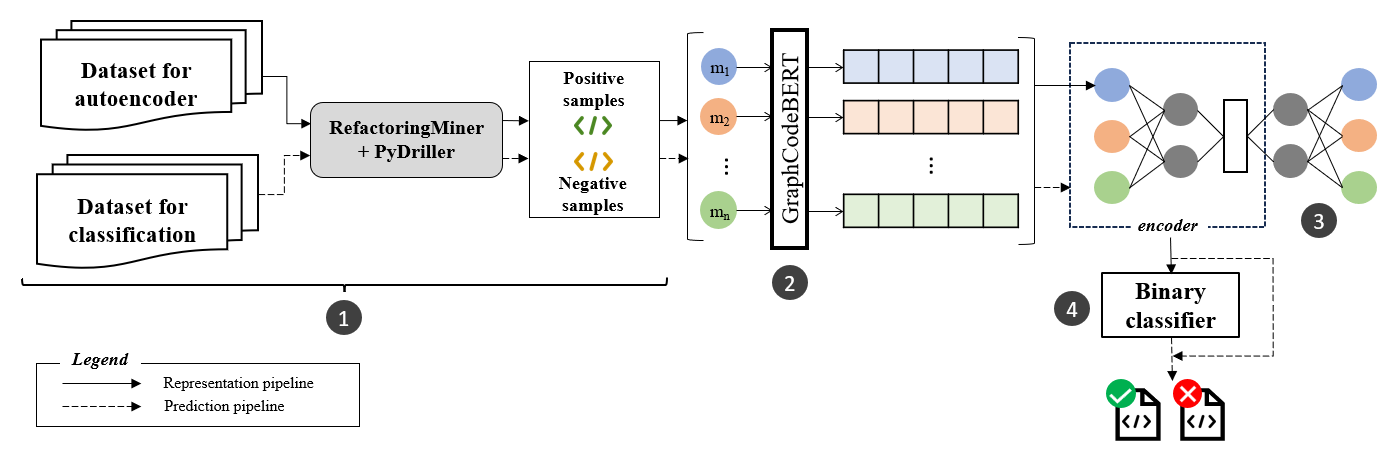
\includegraphics[width=\textwidth]{chapters/identification/Images/ArchDiagram.png}}
\caption{Overview of the proposed approach}
\label{fig:methodology}
% \vspace{-5pt}
\end{figure*}
\subsection{Overview}
The study aims to develop a \dl{}-based \exm{} refactoring candidate identification technique that addresses the deficiencies in the existing studies.
Figure~\ref{fig:methodology} presents an overview of our approach.
We first pick a set of repositories to prepare our dataset.
We use existing tools RefactoringMiner~\cite{Tsantalis:ICSE:2018:RefactoringMiner} and PyDriller~\cite{Spadini2018}, to segregate methods into positive and negative samples.
Our approach utilizes \GCB{} to generate embeddings for each sample.
We employ a \dl{} model based on Autoencoder~\cite{Liou2014Autoencoder} that is used for feature extraction and dimensionality reduction. 
We utilize the encoder component of the trained Autoencoder to generate a lower-dimensional latent space representation from the initially high-dimensional embedding input. 
The representation obtained from the bottleneck layer of Autoencoder is then used as a feature vector to train a \rf{} (\RF{}) classifier on the \exm{} identification task.
We formulate the following research questions.
% to evaluate the effectiveness of the proposed approach. 


\begin{itemize}
    \item [\textbf{RQ1}] 
    \textit{How does our proposed approach perform compared to the state-of-the-art?}
    % \smallskip
\end{itemize}    

    By answering this research question, we intend to evaluate and validate the performance of the proposed approach as compared to the
    % \todo{added -}
    state of the art. 


    \begin{itemize}
    \item 
    [\textbf{RQ2}] \textit{How effectively does the autoencoder extracts features for the classification task?}
\end{itemize}    
    In this research question,
    we aim to evaluate the effectiveness of the employed autoencoder-based model by extracting the learned features and using them for the classification task.


\subsection{Dataset preparation}
\label{dataset_prep}

We utilized a subset of repositories ($5$\%) from the $11,149$ open-source Java repositories used by Aniche~\etal{}~\cite{Aniche2020Effectiveness}, as working with the entire set required extensive computing infrastructure. This initial selection yielded $558$ repositories, from which we excluded repositories that were no longer available on GitHub or lacked any instances of \exm{} refactoring throughout their history. After filtering, we obtained $410$ repositories with at least one \exm{} refactoring performed. 
To leverage a trained autoencoder and using the trained encoder of the autoencoder for the classification task without data leakage, we divided this dataset into two parts: one for autoencoder pipeline with $208$ repositories and the remaining $202$ for the classification pipeline.



% \subsubsection{Dataset preparation}
As shown in step~\circled{1} of Figure~\ref{fig:methodology},
we use RefactoringMiner, a state-of-the-art refactoring detection tool~\cite{Tsantalis:ICSE:2018:RefactoringMiner, Tsantalis:TSE:2020:RefactoringMiner2.0} to prepare our dataset.
This tool reports performed refactorings, if any, 
in each commit within a Java repository's history. 
It provides essential metadata such as the code component involved (\eg{} method start line and end line in the case of \exm{} refactoring) and the associated commit hash. Leveraging this information, we utilize PyDriller~\cite{Spadini2018} to iterate through the identified commits and extract source code of the involved methods.


We identify positive samples where \exm{} refactoring has been applied following the mechanism described above.
Identifying negative samples for \exm{} refactoring is a challenging task. Merely excluding methods not reported by RefactoringMiner is insufficient since the absence of refactoring does not guarantee a method is not a refactoring candidate. Previous work have proposed heuristics-based approaches to address this challenge. For instance, Aniche~\etal{}~\cite{Aniche2020Effectiveness} used a criterion based on the method's modification history, while Yamanaka~\etal{}~\cite{Yamanaka2021RecommendingEM} selected code portions that differ from actual extractions. 
However, these heuristics may introduce noise and create sub-optimal datasets by misclassifying potential \exm{} candidates.

We propose a new mechanism to identify negative samples for the study. A method is considered a negative sample in commit $C_{n}$ if it underwent \exm{} refactoring in its parent commit $C_{n-1}$.  
The rationale behind this idea is that it is highly unlikely that a method that underwent \exm{} refactoring will again go through the same refactoring. This reduces the risk of false negative detection and ensures a high quality dataset. 
The aforementioned approach of identifying positive and negative samples, resulted in $27\small,634$ and $27\small,796$ samples for training and evaluating the Autoencoder, and  binary classifier respectively. Table~\ref{tab:ident_dataset_stats} describes the dataset statistics used to train, test and validate our approach.

\begin{table}[ht!]
    \centering
    \caption{Dataset statistics} \label{tab:ident_dataset_stats}
        \begin{tabular}{cccc|cccc}
            \toprule
            \multirow{2}{*}{Dataset} & \multicolumn{3}{c}{Positive samples} & \multicolumn{3}{c}{Negative samples} \\
            \cmidrule(lr){2-7}
& \makecell[c]{Avg.\\ LOC} &  \makecell[c]{Avg. \\ token\\ length} &  \makecell[c]{Median \\ LOC} &  \makecell[c]{Avg.\\ LOC} &  \makecell[c]{Avg.\\ token\\ length} &  \makecell[c]{Median \\ LOC} &\\
            \cmidrule(lr){1-7}
\makecell[l]{Train split}& $36.46$ & $343.26$ & $14$ & $26$ & $25.23$ & $263.24$\\ \addlinespace
\makecell[l]{Test split} & $36.22$ & $341.57$ & $14$ & $26$ & $24.46$ & $261.55$ \\ \addlinespace
\makecell[l]{Val split} & $35.57$ & $338.88$ & $13$ & $26$ & $25.50$ & $268.27$ \\ \addlinespace
% \makecell[l]{$\mathcal{D}$} & 411.68 & 447.69 & 185.94 & 241.88 \\ 
            \bottomrule
        \end{tabular}    
\end{table}
\vspace*{\fill}


\subsection{Data representation}

In step~\circled{2}, we use \GCB{} to capture both syntactic and semantic information of code, providing a comprehensive representation of code snippets by using graph-guided masked attention function to incorporate the code structure. 
The initial step in processing the input code through the \GCB{} model involves tokenization and encoding. To accomplish this, we utilize the pre-trained \GCB{} tokenizer.
% The \GCB{} model anticipates an input sequence of tokens, which must begin with a special \texttt{[CLS]} token and conclude with another special token, \texttt{[SEP]}. 
To ensure the token sequence adheres to the model's maximum length of $512$, we truncate it if it surpasses this limit. 
Subsequently, we perform batch encoding on the token sequence, generating \texttt{input\_ids} which represent the tokens numerically for the model. 

To extract the embeddings, we pass this encoded input to \GCB{}. 
During the forward propagation of the input, each of the $12$ hidden layers of the model generates individual token embeddings based on the surrounding context. To get the condensed representation of the sequence of tokens, we use mean pooling. We conducted a pilot study and we found that this approach performs better than taking the embedding of the \texttt{[SEP]} token alone.
This results in a single embedding vector of size $768$ for each of the input sample. We consider this as our feature vector for the classification task.

% \vspace{-1mm}

\subsection{Model training and classification}


\subsubsection{Autoencoder}

We use the generated embeddings from \GCB{} as the input for training the autoencoder model (step~\circled{3}). 
The architecture of the autoencoder that we trained consists of an encoder with three fully connected linear layers and ReLU activation to learn the hidden representation that reduces the input dimension to a bottleneck layer of size $128$. The decoder reverses this process to reconstruct the original input of size $768$. The autoencoder model is trained on $70\%$. The rest $30\%$ is used to validate the model. We calculate the reconstruction loss using \textit{Mean Squared Error} (MSE) loss.


\subsubsection{Binary classifier}
After training the autoencoder, in step~\circled{4}, we take the \textit{encoder} part of the trained model and use it as our feature extractor for the binary classification dataset.
We train two classifiers---a traditional machine learning model \rf{} and a \dl{}-based feed forward neural network, and compare their performance. 
We chose to use \rf{}
due to its ensemble learning method for classification and its ability to learn the non-linear relationship between the features,
\rf{} has shown to perform very well in different software engineering tasks~\cite{DiNucci2018, Immaculate2019} including refactoring identification~\cite{Aniche2020Effectiveness,VanDerLeij2021Data}. 

To train our models, 
we first split the $27,796$ samples into train, validation, and test sets in $70:10:20$ ratio 
using stratified sampling. 
We use \textit{GridSearchCV}
to select the optimal hyper-parameters for \rf{}.
The optimal set of hyper-parameter values along with their search space is reported in Table~\ref{tab:rfparams}
The neural network classifier consists of two fully connected layers with ReLU activation and a final sigmoid activation layer.

\begin{table*}[ht]
\captionsetup{skip=10pt}
\centering
\caption{Optimal hyper-parameter values for random forest}
\label{tab:rfparams}
\rowcolors{2}{gray!25}{white}
\begin{tabular}{p{5cm}%
>{\raggedleft\arraybackslash}p{4cm}%
>{\raggedleft\arraybackslash}p{4cm}%
}
\textbf{Parameter} & \textbf{Search space} & \textbf{Best value} \\ \midrule
Number of trees & ${[}100, 200, 300, 1000{]}$ & $1000$ \\
Minimum samples split    & ${[}8, 10, 12{]}$           & $10$   \\
Minimum leaf node samples              & ${[}3, 4, 5{]}$             & $3$    \\
Maximum features              & ${[}2, 3{]}$                & $2$    \\
Maximum tree depth                    & ${[}80, 90, 100, 110{]}$    & $80$  \\\bottomrule
% \vspace{-5pt}
\end{tabular}
\end{table*}

\subsubsection{Evaluation}

To evaluate our models, we calculate the \textit{accuracy, precision, recall,} and \textit{F1 score}.


Initially, the test split of our classification dataset, 
contains positive and negative samples in equal proportion. 
However, it has been argued~\cite{Sharma2021, DiNucci2018} that a test set not representative of the real-world may show good performance while experimentation 
but do poorly when deployed in a real-world scenario. 
To address this issue, 
we identify the ratio of positive and negative samples in the following manner. 
First, we sample $20$ repositories from our dataset randomly. 
For each of the selected repositories, we identify the commits in which \exm{} refactoring has been applied using RefactoringMiner along with the count of such methods ($posCount$). 
Using PyDriller, we identify the count of total methods present in the source code for that commit ($totalCount$). 
Then we compute the ratio $\frac{posCount}{totalCount}$ and take the mean across all identified commits to find a real-world ratio of \exm{} refactoring candidates. 
We modify the test set  to represent the computed ratio ($85:15$) and then perform the evaluation. 


\section{Experimental Results}
\noindent
\textbf{RQ1}: \textit{How does our proposed approach perform compared to
the state-of-the-art?}




In this research question, we compare our two approaches \texttt{M1} (\ie{} neural network-based classification) and \texttt{M2} (\ie{} \rf{}-based classification), where both the models utilize GraphCodeBERT and Autoencoder to generate latent representation.
We compare the results from our models
against state-of-the-art approach from Aniche \etal{} \cite{Aniche2020Effectiveness}.
Though the baseline study compare many machine learning techniques,
we chose to compare our models with only their \rf{} model because it reported the best results in that study.
All of the models we tested using the same test split.
% as described in Section~\ref{dataset_prep}. 

\begin{table}[ht]
\centering
\caption{Experimental results for RQ1}
\label{tab:exresults}
\rowcolors{2}{gray!25}{white}
\begin{tabular}{p{4cm}|%
>{\raggedleft\arraybackslash}p{2cm}%
>{\raggedleft\arraybackslash}p{2cm}%
>{\raggedleft\arraybackslash}p{2cm}%
>{\raggedleft\arraybackslash}p{2cm}%
}
\textbf{Models} & \textbf{Accuracy} & \textbf{Precision} & \textbf{Recall} & \textbf{F1-score} \\ \midrule
M1 (GraphCodeBERT + Autoencoder + Neural Network) & $0.57$ & $0.71$ & $0.57$ & $0.63$ \\
M2 (GraphCodeBERT + Autoencoder + Random forest) & $\mathbf{0.87}$ & $\mathbf{0.90}$ & $\mathbf{0.87}$ & $\mathbf{0.88}$  \\
Baseline (with random forest) & $0.84$ & $0.44$ & $\mathbf{0.87}$ & $0.58$ \\\bottomrule
\end{tabular}
\end{table}


Table~\ref{tab:exresults} presents results of our experiments.
From the results it is evident that our \texttt{M2} model outperforms the baseline as well as the \texttt{M1} model. 
We observe that both \texttt{M1} and \texttt{M2} outperform the baseline. Specifically, we see that \texttt{M2} outperform the \rf{} used by Aniche~\etal{} by nearly 50\% in terms of precision.
At the same time, our model \texttt{M2} exhibits a good recall rate of $0.87$.
Consequently, we see that our model 
performs significantly better than the considered baseline model by approximately $30\%$ in terms of F1 score.


\begin{boxH}
\textbf{RQ1 Summary:} 
Our results show that our \rf{}-based model outperforms the baseline model significantly (by $30\%$, in terms of F1 score).
The results indicate that our  code representation is successfully capturing syntactic and semantic characteristics of code necessary to identify \exm{} refactoring candidates.
\end{boxH}

\noindent
\textbf{RQ2}: \textit{How effectively does the autoencoder extracts features for the classification task?}
% \vspace{0.3mm}

We train an autoencoder model and use the trained encoder part of it as a feature extractor.
We do so to reduce the vectors' dimensionality and extract relevant features from the embeddings generated from \GCB{}. 

\begin{figure}[htbp]

\begin{minipage}[t]{0.49\linewidth}
    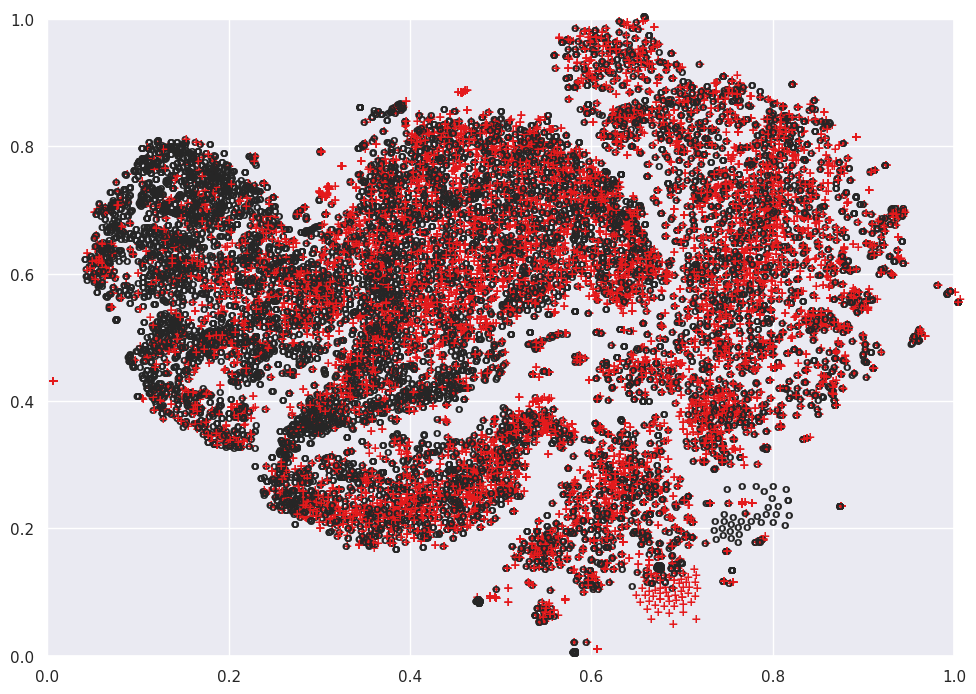
\includegraphics[width=\linewidth]{chapters/identification/Images/tsne_gc.png}
    \caption{Class separation with embeddings (from \GCB{})}
    \label{embonly}
\end{minipage} 
    \hfill%
\begin{minipage}[t]{0.49\linewidth}
    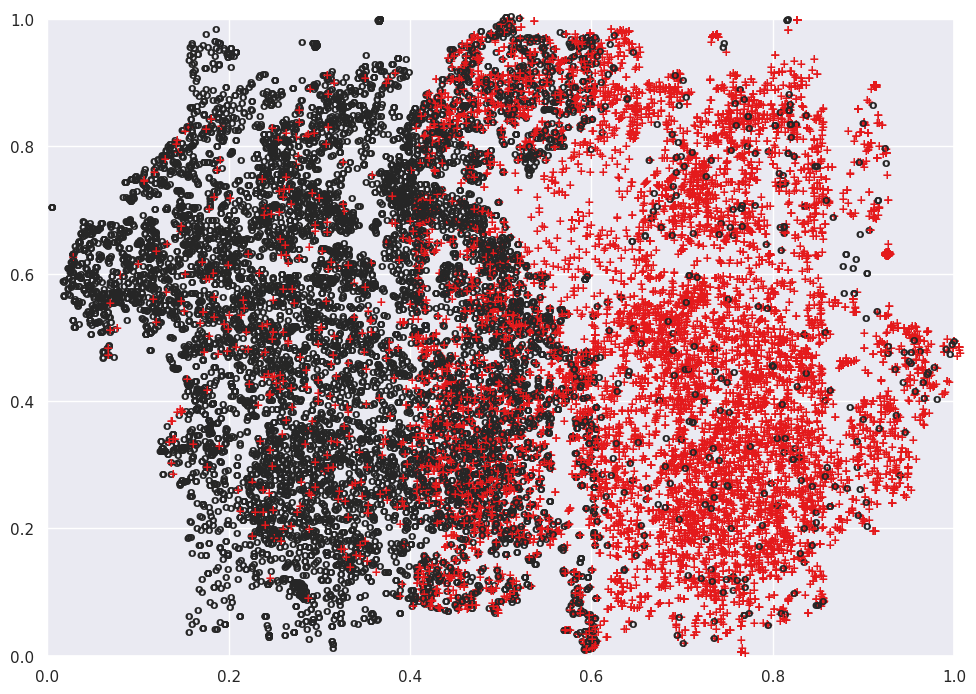
\includegraphics[width=\linewidth]{chapters/identification/Images/tsne_ae_1.png}
    \caption{Class separation with encoded embeddings (from Autoencoder)}
    \label{encodedemb}
\end{minipage}%

\end{figure}


% As we can see from the curve, the model performs well at reconstructing the input embeddings with minimum loss. 
To measure the performance and usefulness of the trained autoencoder model as a feature extractor, we first analyze the \texttt{t-SNE}~\cite{van2008visualizing} plots of the embeddings generated by \GCB{} and those generated by the combination of \GCB{} and Autoencoder. We do so to study the class separability. The distinguishability of classes in the \texttt{t-SNE} space is assessed through a clear separation and quantified by calculating the Euclidean distance between the centroids of each class. Figure~\ref{encodedemb} shows a reasonably clear bifurcation between the classes with an euclidean distance of $0.367$ as compared to $0.122$ for Figure~\ref{embonly}. We can infer that a classification model trained on the encoded embedding will perform better than the one trained on embeddings alone. This observation can be attributed to the autoencoder being able to learn hidden features unique to each type of sample which helps it to segregate them.

To further investigate the effectiveness of these representations, we perform an ablation study where we train classifier with and without the autoencoder representation of the embeddings. 
% In the first case, we train and test the model directly with the embeddings generated by \GCB{}. 
% In another case, after generating the initial embeddings for the training set from \GCB{}, we encode them using the trained encoder part of the autoencoder model. 
We report the performance results in Table~\ref{tab:emcomp}.
% The evaluation metrics are computed and reported in Figure~\ref{fig:aechart} for a comparative analysis. 
The \rf{} classification model, when trained with the encoded representation of the embedding provided by Autoencoder, 
outperforms the one trained with only the \GCB{} embedding vector as features. 
% While we observe a slight increase of \textbf{$7\%$} in terms of Precision metric value, there's a significant increase of about \textbf{$28\%$} on average for the other 3 metrics. 
These findings support our claim that the
autoencoder extracts features and reduces dimensionality effectively
in the context of refactoring candidate identification.

\begin{boxH}
\textbf{RQ2 Summary:} Autoencoder-encoded code representations from \GCB{} significantly improve classification performance compared to \GCB{} representations alone.
\end{boxH}


\begin{table}[h!]
\centering
\caption{Encoded embedding performance}
\label{tab:emcomp}
\rowcolors{2}{gray!25}{white}
\begin{tabular}{p{4cm}|%
>{\raggedleft\arraybackslash}p{2cm}%
>{\raggedleft\arraybackslash}p{2cm}%
>{\raggedleft\arraybackslash}p{2cm}%
>{\raggedleft\arraybackslash}p{2cm}%
}
\textbf{Models} & \textbf{Accuracy} & \textbf{Precision} & \textbf{Recall} & \textbf{F1-score} \\ \midrule
\begin{tabular}[c]{@{}l@{}}Embeddings\end{tabular} & $0.57$ & $0.71$ & $0.57$ & $0.63$ \\
\begin{tabular}[c]{@{}l@{}}Encoded embeddings\end{tabular}  & $\mathbf{0.87}$ & $\mathbf{0.90}$ & $\mathbf{0.87}$ & $\mathbf{0.88}$ 
% Baseline (with random forest) & 0.84 & 0.44 & \textbf{0.87} & 0.58
\\\bottomrule
\end{tabular}
\end{table}

% \section{Related Work}
% % \todo{are there studies that identify refactoring candidate without using machine learning? If yes, we need a subsection for them.}

\subsection{Refactoring candidate identification using traditional techniques}

Software developers can manually decide \textit{what} to refactor according to their intuition and past experiences~\cite{Al2015Identifying}.
Often, they use automated tools to calculate code quality metrics and code smells to identify refactoring candidates~\cite{Mens2004Survey, Al2015Identifying}. 
Another method to identify refactoring candidates is to define a set of preconditions or compliance rules. If a code did not follow these rules, it was considered a candidate for refactoring. Studies by Bois \etal{}~\cite{Du2004Refactoring} and Kataoka \etal{}~\cite{Kataoka2001Automated} used such compliance rules.

Another technique considers creating clustering algorithms to identify if code needs refactoring. 
Czibula \etal{}~\cite{Czibula2008Hierarchical} and Serban \etal{}~\cite{Serban2007Restructuring}, 
created clusters based on the distance between methods and attributes within and outside of classes to identify numerous refactoring candidates.
Similarly, Bavota \etal{}~\cite{Bavota2011Identifying} suggest a graph-based approach that uses weighted graphs instead of abstract syntax trees to identify methods that can be extracted. 
Finally, Tsantalis \etal{}~\cite{Tsantalis2009Identification} used code slices to identify \exm{} candidates.

\subsection{Detecting refactoring with Machine Learning techniques}

Many studies have explored ways to identify refactoring candidates automatically using machine learning.
Typically, such studies use
source code metrics or commit messages to train a model. For example, Aniche \etal{}~\cite{Aniche2020Effectiveness} predict $20$ kinds of refactorings at the method, class, or variable level. 
They use a large number of code, process, and ownership metrics to train six supervised machine learning algorithms. 
The study reports that \rf{} model performs the best among the compared models.
Gerling~\cite{Gerling2020Machine} conducted an empirical study as an extension of Aniche \etal{}'s study. 
They focused on improving the data collection process in Aniche \etal{}'s study to create a high quality large-scale refactoring dataset. 


Similarly, Van Der Leij \etal{}~\cite{VanDerLeij2021Data} analyze five machine learning models to predict \exm{} refactoring and compare the results with industry experts.
They collect $61$ code metrics and analyze \rf{}, \dt{}, \logr{}, Linear \SVM{}, and Gaussian \nb{} algorithms. 
They found \rf{} as the best performing model. 
Kumar \etal{}~\cite{Kumar2019Method} perform a study to predict method-level refactoring and analyze $10$ machine learning classifiers. 


Sagar \etal{}~\cite{Sagar2021Comparing} considers the problem of refactoring candidate prediction as a multi-class classification problem. 
Their study uses source code quality metrics and commit messages as features to predict six method-level refactorings. 
They compare two machine learning models: a text-based model that analyses keywords from commit messages and a source code-based model that analyses $64$ code quality metrics. 
Kurbatova \etal{}~\cite{Kurbatova2020Recommendation} use code embeddings generated from Code2Vec~\cite{Alon2019Code2vec} to train their machine learning model to predict the \mm{} refactoring. 



\section{Threats to Validity}
\noindent
\textbf{Construct validity:} 
Construct validity measures the degree to which tools and metrics actually measure the properties that they are supposed to measure. 
It concerns the appropriateness of observations and inferences based on measurements taken during the study.
The quality of positive and negative samples extracted from RefactoringMiner and PyDriller poses a threat to validity.
Though RefactoringMiner and PyDriller are state-of-the-art tools that are widely used and considered accurate,
to mitigate the threat,
we randomly picked up a subset of the identified negative samples and manually evaluated the quality of the samples.


Our approach uses a significantly smaller dataset (approximately $5\%$) compared to the dataset used in the state-of-the-art approach.
Though the chosen repositories are representative,
it can be considered a threat to validity.
We chose the smaller dataset
because of the computing resources required for the full-size dataset. 
Additionally, in this study, we aimed to explore the feasibility and effectiveness of the proposed approach.
In the future, we aim to repeat the experiment with a larger dataset.

\noindent
\textbf{External validity:}
External validity concerns the generalizability and repeatability of the produced results.
One of the threats to validity in this thesis is that the approach proposed is exclusive to \exm{} refactoring. 
Using our approach for another kind of refactoring is challenging and requires extensive reworking of the approach used. 
For example, \emph{move method} refactoring moves a method to an appropriate class~\cite{Fowler1999Refactoring}. 
We cannot apply the same approach that we adopted to create \exm{} dataset for \emph{move method} refactoring
because we will not have the code to collect in the refactored commit since the method would have moved to another class. 
A similar challenge is expected when considering other refactoring types, such as \emph{pull up method} and \emph{push down method}.
In the future, we would like to address this challenge and propose an effective and generic dataset-creation approach for different refactoring types.


\chapter{Comparing Reinforcement Learning and Supervised Learning in generating refactored code accurately}
\epigraph{Learning without thought is labour lost; thought without learning is perilous.}{--- \textup{Confucius}}

In this chapter, we present an innovative approach that combines reinforcement learning with large language models to fully automate the extract method refactoring process. Our method addresses key limitations of current tools by considering code-specific requirements during the refactoring process. The results show notable improvements in both automated metrics and practical code functionality, demonstrating the potential for reducing manual developer effort in code maintenance.


\section{Introduction}
% \noindent
% \section{Introduction}
Refactoring is an important software development activity that employs various techniques to enhance the structure and quality of source code without altering its functionality~\cite{Opdyke1992Refactoring, Fowler1999Refactoring}. 
By removing code smells~\cite{Fowler1999Refactoring} the practice aims to improve maintainability, encapsulating quality attributes such as readability, flexibility, and testability~\cite{ieee1990standard, chawla2015sqmma}.
Refactoring helps maintain high code quality, facilitating long-term maintainability and evolution~\cite{moser2007case}. 

% A major cause for poor code quality is code smells. Code smells are surface-level indicators that often signal deeper, underlying issues within a software system~\cite{Fowler1999Refactoring}. These smells can appear in various forms, such as implementation, design, and architectural smells. While not necessarily problematic on their own, they serve as warning signs of more significant concerns in the codebase. To address these smells and enhance software quality, developers utilize various refactoring techniques. These techniques are tailored to target specific types of smells, aiming to eliminate or mitigate the underlying problems they represent. Singh and Kaur~\cite{singh2018systematic} provide a comprehensive systematic study on this topic, offering valuable insights into different code smells and the most effective refactoring approaches for each.

\Exm{} refactoring is one of the most commonly applied refactoring techniques that involves moving a coherent code fragment from a method into a new, aptly named method~\cite{Fowler1999Refactoring}.
By creating cohesive and smaller methods, extract method refactoring not only improves code quality and maintainability but also serves as a foundation for more complex refactoring operations~\cite{Zarras2015}. 
Extract method refactoring constitutes a significant proportion, approximately $49.6$\%, of the total refactoring recommendations generated by JDeodorant~\cite{JDeodrant}, a widely recognized tool for supporting extract method operations. Furthermore, this refactoring technique has been acknowledged as a crucial operation by both open-source developers~\cite{silva2016we} and industry practitioners~\cite{van2021data}, underscoring its importance in software maintenance.

Automatically performing extract method refactoring, consist of two major steps~\cite{kramer2010legacy}. 
First, \textit{identification} of a candidate method that requires extract method refactoring; 
and second, intelligently \textit{extracting} the logic and \textit{forming} a new method with appropriate parameters, without human intervention. 
% A crucial aspect of software development involves determining whether a source code entity requires refactoring and, if so, identifying the most appropriate refactoring technique for the given context. 
For the first step,
\ie{} identifying a candidate method for the refactoring,
practitioners often rely on intuition and experience.
They also utilize automated tools to assess code quality metrics and detect code smells~\cite{Sharma2018} to get aid in the decision process.
% TS: commented the following because that's not the focus of this study.
% However, these metrics and smell detection mechanisms primarily focus on problem identification, offering limited guidance on the necessity and selection of specific refactoring techniques to address the identified issues or enhance code quality metrics. In recent years, there has been significant progress in automatically identifying refactoring candidates using static metrics and source code properties~\cite{aniche2020effectiveness, karakati2023software} and also intelligent techniques involving machine learning. 
The second step of automated extract method refactoring involves comprehending and extracting source code into a new method. Several approaches have been proposed to address this challenge. Hubert~\cite{hubert2019implementation} developed a method for generating extract method refactoring candidates using static code analysis tools. Maruyama~\cite{hubert2019implementation} proposed a candidate generation technique utilizing block-based slicing. Shahidi \etal{}~\cite{shahidi2022automated} introduced an algorithm for identifying, generating, and ranking extract method candidates through graph analysis. However, these approaches exhibit a few limitations. 
Specifically, most of these approaches require the developers to manually identify the bounds of a block to be refactored \ie{} start and end statements,
to perform the refactoring.
Such a reliance on human knowledge reduces the efficacy and significance of automated refactoring.
Furthermore, static analysis and metric-based methods often fail to capture latent contextual and syntactical code characteristics that could enhance the refactored code.
For instance, these approaches do not offer meaningful identifiers for the new method and its parameters.
% \todo{limitations of the existing approaches is very weak. - The end of next para also has few limitations}

The emergence of \llm{}s (\llmsc{}s)
has enabled the convenience in generative tasks, including code generation with high accuracy ~\cite{wang2021codet5identifierawareunifiedpretrained, ahmad2021}.
% The automated generation of methods following Extract Method refactoring can be conceptualized as a text generation task. Recently, the research community has observed a significant surge in studies employing code \Llm{}s (\llmsc{}s) for text generation. 
The field of code generation has seen significant advancements recently, with pre-trained language models such as GitHub Copilot~\cite{githubGitHubCopilot} and Amazon Q Developer~\cite{amazonCodingAssistant} demonstrating impressive capabilities.
Though such \llmsc{} perform well on many text and code generation tasks, they show mediocre performance for tasks requiring domain-specific or uncommon knowledge. 
For example, \llmsc{} have shown proficiency in generating code for known and common problems but they struggle with unfamiliar problems~\cite{chen2021evaluating}. 
Similarly, in our context,
current \llmsc{} can generate refactored code but often omit the contextual information or generate incomplete, broken, or even uncompilable code~\cite{jha2023codeattack}.
% However, these achievements come with challenges. The process of pre-training language models on extensive code databases is resource-intensive, making it unfeasible for many academic institutions and small companies with limited computational power~\cite{huang2023not}.
Moreover, using third-party code completion services raises privacy concerns for many organizations. A notable example is Samsung Electronics~\cite{JaiVijayan_2023}, which reportedly experienced three data leakage incidents while using online code completion tools such as ChatGPT. These issues highlight the growing need for developing task-specific code generation models. 
% Such models, based on fine-tuning techniques, could be tailored for personal or organizational use, addressing both resource constraints and privacy concerns.

Language models for code are sequence-to-sequence models pre-trained on large corpus of code
and can be fine-tuned for various software engineering tasks, including code summarization~\cite{ahmed2022few, sun2024source}, translation~\cite{eniser2024towards, yin2024rectifier}, completion~\cite{bairi2024codeplan, eghbali2024hallucinator}, bug localization~\cite{yang2024large}, vulnerability detection~\cite{lu2024grace, zhou2024large}, and program repair~\cite{Sharma2024}.
Despite these advancements,
to the best of our knowledge, 
the application of language models for code refactoring remains largely unexplored. 
Inspired by applying \llmsc{}s on a variety of software engineering tasks, there has been some attempts to generate refactored code using them.
For example, a recent contribution by Pomian \etal{}~\cite{Pomian2024} introduced EM-Assist, an IntelliJ IDEA plugin that leverages \llmsc{}s to generate and rank refactoring suggestions using few-shot prompting. 
% \todo{Are they \textbf{generating} code} \todo{- OpenAI API is generating the suggestions but they statically preprocess the suggestions heavily, e.g., using program slicing before applying it.}
% Fine-tuning is another common technique to train a pre-trained model for a specific downstream task.
% However, EM-Assist employs few-shot prompting for the generation of extract method names, which may have limitations. In contrast, fine-tuning a model for a specific task such as \exm{} refactoring potentially allows for more precise adaptation, potentially yielding consistently superior performance compared to few-shot prompting techniques. Furthermore, it is noteworthy that the aforementioned tool solely generates method names, necessitating manual intervention from developers to select the code segments for extraction. This limitation underscores the need for more comprehensive automated solutions in the field of code refactoring. 

Fine-tuning is another common technique to train a pre-trained model for a specific downstream task.
% Recent studies have highlighted significant limitations in existing approaches to automatic code generation, particularly in the context of refactoring. 
While fine-tuning pre-trained code language models appears to be a promising solution, it has been observed that a considerable portion of programs generated by these models often fail to pass unit tests~\cite{chen2021evaluating, li2022competition, jha2023codeattack}.
Such challenges deter the adoption of the automated refactoring tools and methods.
% This is particularly problematic for extract method refactoring, where maintaining the functionality of the method or class is paramount.

To address these challenges, we evaluate performance of fine-tuned models and
propose a deep reinforcement learning approach that aligns fine-tuned code language models to generate refactored code by applying extract method refactoring automatically. 
% Our approach builds upon recent advancements in reinforcement learning for code generation and completion, such as the work by Wang \etal{}~\cite{wang2022compilable} on generating compilable code with compiler feedback, CodeRL by Lee \etal{}~\cite{le2022coderl}, PPOCoder by \etal{}~\cite{shojaee2023execution}, and IRCoCo by Li \etal{}~\cite{li2024ircoco}. 
% Our framework encompasses several key steps. 
% We begin by utilizing the SEART tool to collect repositories and employ RefactoringMiner to identify methods for refactoring. 
Our approach, first, creates a dataset using state-of-the-art tools such as RefactoringMiner~\cite{Tsantalis:ICSE:2018:RefactoringMiner, Tsantalis:TSE:2020:RefactoringMiner2.0}.
We use the dataset to fine-tune four language models, pre-trained on code, using Supervised Fine Tuning (\sft{})~\cite{howard2018universal, kenton2019bert}
% \todo{cite}. 
% Initial evaluation using metrics such as BLEU and CodeBLEU showed promising results. However, qualitative analysis revealed that only $33$\% of the generated methods passed their corresponding unit tests, highlighting the limitations of the SFT approach for code generation tasks.
To enhance model performance and better align it with the objective of generating compilable code while preserving functionality, we use Proximal Policy Optimization (PPO)~\cite{schulman2017proximal} for reinforcement learning optimization.

Our reinforcement learning approach utilizes an actor-critic architecture~\cite{konda1999actor, wan2018improving}, where the actor component generates refactored code, and the critic component assesses the quality of the generated code. This architecture enables the model to learn more efficiently in the complex space of code refactoring by providing guidance on the desirability of different refactoring decisions.
The critic component incorporates discrete, non-differentiable reward signals in three stages. We first check for syntactic correctness, then assess whether the code compiles successfully, and finally, we use RefactoringMiner to detect if the desired refactoring has been applied.

To strike a balance between generating refactorings and maintaining the knowledge gained during supervised fine-tuning, we introduce a Kullback-Leibler (KL) divergence~\cite{kullback1997information, shojaee2023execution} term in the reward function. This term measures the difference between the model's current behavior and its initial behavior learned during supervised fine-tuning. By incorporating this term, we encourage the model to explore new refactoring strategies while preventing it from deviating too far from its initial understanding of code refactoring. 

Our study yielded promising results. 
The \plbart{} model,
when fine-tuned using supervised learning,
demonstrates superior performance among the chosen models
when evaluated using conventional metrics such as \bleu{},
\rouge{}, and \codebleu{}.
However, \codetf{} outperforms other models when trained with deep reinforcement learning.
\textbf{We observe that combining supervised fine-tuning with deep reinforcement learning prove most effective},
compared to fine-tuning the models or training using reinforcement learning individually.
Qualitative evaluation further validates that the combination works the best, exhibiting enhanced syntactic accuracy, compilation rates, and unit test performance. 

We list the key contributions of this thesis below.
\begin{itemize}
    \item We evaluate the effectiveness of supervised fine-tuned models for automatic \exm{} refactoring.
    The approach addresses the limitations of existing approaches such as manual code selection to specify the code block to-be extracted.
    \item The study presents a hybrid method that combines supervised fine-tuning with reinforcement learning optimization, specifically tailored for extract method refactoring tasks. We then evaluate the approach both quantitatively and qualitatively to ensure that it generates syntactically and semantically accurate refactorings.
    \item This study also contributes a tool for analyzing Java repositories on GitHub to create an extract method refactoring datasets with associated metadata. We provide the tool and the dataset created using it for replication and extension purposes.
\end{itemize}


% \section{Background}
% 
\epigraph{Research is to see what everybody else has seen, and think what nobody has thought.}{--- \textup{Dr. Albert Szent-Gyorgyi}}

This chapter has two main sections. The first section provides the background concepts needed to understand our research. The second section reviews existing research in this field, examining prior work that shapes the basis of our study.

\section{Context}

\subsection{Extract method refactoring}
Extract Method refactoring, first formalized by Fowler \cite{Fowler1999Refactoring}, is a fundamental technique for improving code maintainability by decomposing large methods into smaller, more focused units. This transformation involves identifying cohesive code fragments and extracting them into new methods while preserving program behavior \cite{murphy2011we}. Recent studies by Silva~\etal{} \cite{silva2016we} and Tsantalis~\etal{} \cite{Tsantalis2018Accurate} have shown that Extract Method is among the most frequently applied refactorings in practice, accounting for approximately 15-25\% of all refactoring operations in large-scale systems.

The primary motivation for Extract Method refactoring is to address the``Long Method" code smell, where methods become long, complex or incohesive, violating the single responsibility principle \cite{martin2009clean}. The process involves identifying a coherent fragment of code, extracting it into a new method with an appropriate name, and replacing the original fragment with a call to the newly created method. This transformation must preserve program semantics while managing variable scope, parameter passing, and return values \cite{kim2012field}. Studies by Murphy-Hill et al. \cite{murphy2011we} have shown that while developers frequently perform this refactoring manually, automated tool support remains challenging due to the complexity of ensuring behavioral preservation and identifying optimal extraction points.

\subsection{Embeddings}

Code embeddings are dense vector representations that capture semantic properties of source code in a continuous space. Alon~\etal{} \cite{Alon2019Code2vec} introduced Code2Vec, demonstrating how path-based attention over abstract syntax trees can create meaningful code representations. This was further advanced by Feng~\etal{}. \cite{feng2020codebert} with CodeBERT, which combines both structural and textual features of code. These embedding techniques have revolutionized code analysis by enabling deep learning models to better understand and process source code semantics.

Recent advancements in code embeddings have focused on incorporating multiple views of code, such as data flow, control flow, and natural language documentation. Guo et al. \cite{guo2022unixcoder} demonstrated that unified representations combining these different aspects significantly improve performance on some downstream tasks. The effectiveness of these embeddings has been particularly evident in tasks such as code similarity detection, bug localization, and automated program repair \cite{zhou2019devign}. Furthermore, studies by Kanade~\etal{} \cite{kanade2020learning} have shown that pre-training on large code corpora can create embeddings that capture rich semantic relationships between different programming concepts and patterns.

\subsection{Transformers}

The Transformer architecture, introduced by Vaswani~\etal{} \cite{vaswani2017attention}, revolutionized sequence processing through its self-attention mechanism. In the context of code processing, Ahmad~\etal{} \cite{ahmad2021} demonstrated how Transformers can effectively capture long-range dependencies in source code, while Hellendoorn~\etal{} \cite{hellendoorn2019global} showed their effectiveness in modeling code structure through global attention patterns. The architecture's ability to process sequences in parallel while maintaining contextual relationships has made it particularly suitable for code analysis tasks.

The key innovation of Transformers lies in their self-attention mechanism, which allows the model to weigh the importance of different parts of the input sequence dynamically. For code processing, this is particularly valuable as it enables the model to capture relationships between distant parts of the code, such as variable declarations and their uses, or function calls and their definitions \cite{wang2019self}. Recent adaptations of the Transformer architecture for code, such as CodeT5 \cite{wang2021codet5identifierawareunifiedpretrained}, have introduced specialized attention patterns that better align with code structure, including syntax-aware attention and hierarchical representations that respect code's abstract syntax tree structure.

% \subsection{Large Language Models}

\subsection{Supervised fine-funing of large language models}


Supervised fine-tuning is an add-on training for adapting pre-trained large language models (LLMs), such as CodeT5~\cite{wang2021codet5identifierawareunifiedpretrained}, to specialized tasks. 
This adaptation is achieved by training the models on domain-specific datasets, which is particularly important for enhancing their performance in tasks such as extract method refactoring. In this context, we focus on two predominant model architectures: \textit{encoder-decoder} and \textit{decoder-only} models.

Encoder-decoder models consist of two main components. 
The encoder processes the input sequence (\ie{} source code, in our case) to create a context-rich representation, which the decoder then uses to generate the output sequence (refactored code with extracted method, in our case).
This architecture is particularly useful when the input is a code snippet, and the output is the corresponding refactored version. 
The fine-tuning objective for encoder-decoder models aims to maximize the conditional probability of the correct output sequence given an input sequence. 
% During training, inputs are fed into the encoder, and their corresponding target outputs into the decoder. 
A technique called teacher forcing is employed, where the correct output token from the previous time step is fed as input to the next step. 
% \todo{rewrite this using autoregressive characteristic - I am not sure if enc-dec models have autoregressive characteristics. Do you mean the autoregressive characteristics of the decoder?}

Decoder-only models, such as those used in GPT-like architectures~\cite{radford2019language}, operate differently. They generate each token of the output sequence directly, conditioned on all previous tokens and the input sequence, without a separate encoding phase. The training process involves presenting the combined sequence of the input code and the refactored code to the model, typically separated by a special token, \eg{} ~\textsc{[sep]}.

For both architectures, the loss function commonly used is the cross-entropy loss, calculated over the output sequence tokens. This loss function helps the model learn to predict the correct tokens in the output sequence. 


\subsection{Reinforcement learning for sequence generation}

Reinforcement Learning (\rl{}) is a branch of machine learning focused on 
% teaching algorithms to make a series of decisions~\cite{shakya2023reinforcement}.
training agents to take actions in an environment to maximize some notion of cumulative reward often involving a series of decisions~\cite{shakya2023reinforcement}. 
It uses a model known as the Markov Decision Process (MDP)~\cite{puterman2014markov}, which deals with decision-making where each action is determined by steps, and outcomes are influenced by randomness. 
In \rl{}, an agent (\ie{} an autonomous entity that takes action in the given environment)
improves its decisions through trial-and-error interactions with its environment, learning from the rewards it receives based on its actions. The agent's decision-making strategy is known as the \textit{policy}, which determines the next action to take given the current situation or \textit{state}. The \textit{state} represents the current context or input on which the agent bases its decisions.


In the context of language models, \rl{} can be employed as a training mechanism. 
Here, the language model serves as the \textit{policy}, and the current text sequence is the \textit{state}. 
The model generates an action,
the next word or token,
altering the state into a new text sequence. 
The quality of the completed text sequence determines the reward, assessed either by human judgment or a trained reward model based on human preferences.

Formally, MDP can be defined as follows.

\textbf{State Space: }
The state space \(S\) is the set of all possible language representations up to a maximum length \(L\):
\begin{equation}
    S = \{s \mid s \in \mathbb{R}^d \times l, l \leq L\}
\end{equation}
where \(d\) is the dimensionality of the token embeddings and \(l\) is the current sequence length.

% \subsubsection{Markov Decision Process Definition}
\textbf{Action Space: }
The action of the model (actor) is to generate the next token based on the previously generated tokens and the input data. The action space is the vocabulary of the language model, representing all possible tokens:
\begin{equation}
    A = \{1, 2, \ldots, V\}
\end{equation}
where \(V\) is the vocabulary size.

\textbf{State Transition Function: } 
The state transition function \(P\) describes how the environment moves from one state to another given an action. In our sequence generation task, this transition is deterministic:
\begin{equation} \label{eq:state_trans_func}
    P(s_{t+1} \mid s_t, a_t) = 
    \begin{cases} 
    1 & \text{if } s_{t+1} = [s_t; e(a_t)], \\
    0 & \text{otherwise}
    \end{cases}
\end{equation}
where \(e(a_t)\) is the embedding of the chosen token.

\textbf{Policy: }
The policy is represented by a language model that produces a probability distribution over the next token given the current state:
\begin{equation}
    \pi_\theta(a \mid s) = \text{LM}_\theta(a \mid s)
\end{equation}
where \(\text{LM}_\theta\) is the language model with parameters \(\theta\).

\textbf{Value Function: }
The value function estimates the expected cumulative reward from a given state under a particular policy:
\begin{equation}
    V_\phi(s) = \mathbb{E}_{\pi_\theta}\left[\sum_{t=0}^{\infty} \gamma^t R_t \mid S_0 = s\right]
\end{equation}
where \(\phi\) are the parameters of the value head and \(\gamma\) is the discount factor.

\subsubsection{Reward}
In sequence modeling, the reward quantifies the quality or desirability of generated sequences. It measures how well the generated sequence aligns with desired characteristics, such as fluency, coherence, or task-specific objectives.

\subsubsection*{Reward Function}
The reward function \(R\) can be expressed as:
\begin{equation}
    R(s, a) = \lambda_1 r_{\text{task}}(s, a) + \lambda_2 r_{\text{seq}}(s, a)
\end{equation}
where $r_{\text{task}}$ represents task-specific evaluation metrics, $r_{\text{seq}}$ captures sequence quality measures, and $\lambda_1$, $\lambda_2$ are weighting coefficients balancing different reward components..


In the software engineering domain, \rl{} has been used for code completion tasks~\cite{shojaee2023execution, li2024ircoco} and code summarization~\cite{wan2018improving}. They all use actor-critic methods to train the language models for specific downstream tasks. The actor is the policy model, the main language model pre-trained or fine-tuned on code data and the critic is another component that evaluates the output generated by the actor and provides a reward signal. Based on this architecture, we formulate our problem as follows. 


\subsection{Solution framework}

In this second part of this thesis, we focus on aligning a fine-tuned large language model for extract method refactoring generation using Proximal Policy Optimization (\ppo{})~\cite{schulman2017proximal}---a popular actor-critic  reinforcement learning method. 
This alignment process involves several key components: the actor, the critic, rewards, the value function, and KL divergence.

The \textit{actor} in our setting is the language model itself, which generates sequences of code such as extracting methods from code snippets. It takes the current code as input and outputs a refactored version with extracted methods. The \textit{critic} is a separate component that evaluates the quality of the refactoring produced by the actor, providing a score or reward that reflects how well the generated refactoring meets the desired criteria, such as syntactically and semantically accurate refactored code.

A \textit{reward} is a numerical score assigned to each generated refactoring, indicating its quality. Higher rewards are given for refactorings that improve code properties, while lower rewards indicate poor refactoring outcomes, such as introduction of errors. These rewards guide the actor in learning to generate more desirable refactorings over time.

The \textit{value function} estimates the expected reward from a given state or step in the sequence generation process. It predicts how good the current refactoring is, considering future rewards. In practice, the value function is represented by a separate neural network head, called a \textit{value head}, which outputs a scalar value for each input state, estimating the expected cumulative reward, denoted as 
\begin{equation} \label{eq:value_func}
 V(s) = \mathbb{E} \left[ R \mid s \right], where\ R\ is the\ total\ reward
\end{equation}

\textit{Proximal Policy Optimization (\ppo{})} is the algorithm used to train the actor model. \ppo{} optimizes the model's parameters by adjusting its behavior in small, controlled steps, ensuring that changes are not too drastic. This balance between exploration (trying new refactoring strategies) and stability (maintaining effective behaviors) helps the model learn efficiently without losing its learned knowledge.

The \textit{objective function} in PPO aims to maximize the expected reward while ensuring that updates to the policy (the actor's behavior) are not excessively large. The PPO objective can be formulated as:

\[
L^{\text{PPO}}(\theta) = \mathbb{E} \left[ \min \left( r_t(\theta) \hat{A}_t, \, \text{clip}(r_t(\theta), 1 - \epsilon, 1 + \epsilon) \hat{A}_t \right) \right],
\]

where \( \theta \) represents the model parameters, \( r_t(\theta) = \frac{\pi_\theta(a_t \mid s_t)}{\pi_{\theta_{\text{old}}}(a_t \mid s_t)} \) is the ratio of the new policy to the old policy, \( \hat{A}_t \) is the advantage estimate, and \( \epsilon \) is a small constant controlling the clipping range.

%  

The \textit{PPO loss} combines the clipped objective function with the value function loss and an entropy bonus. The complete loss function can be expressed as:

\[
L(\theta) = L^{\text{PPO}}(\theta) - c_1 \cdot \text{Value Loss}(\theta) + c_2 \cdot \text{Entropy Bonus}(\theta),
\]

where the \textit{Value Loss} measures the accuracy of the critic's value estimates, and the \textit{Entropy Bonus} encourages exploration by preventing the actor from becoming overly deterministic.

\textit{KL Divergence} (Kullback-Leibler divergence) measures the difference between the old policy $\pi_{\theta_{old}}$ and the updated policy $\pi_\theta$, ensuring that updates to the policy do not deviate excessively from the original behavior. It is calculated as:

\begin{equation} \label{eq:kl_div}
\text{KL}(\pi_{\theta_{old}} \parallel \pi_{\theta}) = \sum_{x} \pi_{\theta_{old}}(x) \log \left( \frac{\pi_{\theta_{old}}(x)}{\pi_{\theta}(x)} \right),
\end{equation}

where $\pi_{\theta_{old}}(x)$, $\pi_\theta(x)$ represent the probability distributions over the possible code refactoring actions that the model can take at a given step.

In summary, the actor generates refactoring suggestions, and the critic evaluates them using static non differential rewards that provide feedback on their quality. \ppo{} optimizes the model's behavior gradually, guided by the value function, the objective function, and loss components, 
% \doubt{I haven't included the objective and loss components because it was very difficult to explain without complex math equations. Should I do it or remove it since it might be understood from just PPO? \\
% If they are short equation, you can. Otherwise, mention them using words.}, 
while KL divergence ensures that changes remain within reasonable limits. This framework enables the fine-tuning of the language models to produce high-quality code refactorings over time.


\section{Related Work}

\subsection{Refactoring candidate identification using traditional techniques}

Software developers can manually decide \textit{what} to refactor according to their intuition and past experiences~\cite{Al2015Identifying}.
Often, they use automated tools to calculate code quality metrics and code smells to identify refactoring candidates~\cite{Mens2004Survey, Al2015Identifying}. 
Another method to identify refactoring candidates is to define a set of preconditions or compliance rules. If a code did not follow these rules, it was considered a candidate for refactoring. Studies by Bois \etal{}~\cite{Du2004Refactoring} and Kataoka \etal{}~\cite{Kataoka2001Automated} used such compliance rules.

Another technique considers creating clustering algorithms to identify if code needs refactoring. 
Czibula \etal{}~\cite{Czibula2008Hierarchical} and Serban \etal{}~\cite{Serban2007Restructuring}, 
created clusters based on the distance between methods and attributes within and outside of classes to identify numerous refactoring candidates.
Similarly, Bavota \etal{}~\cite{Bavota2011Identifying} suggest a graph-based approach that uses weighted graphs instead of abstract syntax trees to identify methods that can be extracted. 
Finally, Tsantalis \etal{}~\cite{Tsantalis2009Identification} used code slices to identify \exm{} candidates.

\subsection{Detecting refactoring with Machine Learning techniques}

Many studies have explored ways to identify refactoring candidates automatically using machine learning.
% The most well-known techniques in automatically predicting refactoring using machine learning 
Typically, such studies use
source code metrics or commit messages to train a model. For example, Aniche \etal{}~\cite{Aniche2020Effectiveness} predict $20$ kinds of refactorings at the method, class, or variable level. 
They use a large number of code, process, and ownership metrics to train six supervised machine learning algorithms. 
The study reports that \rf{} model performs the best among the compared models.
Gerling~\cite{Gerling2020Machine} conducted an empirical study as an extension of Aniche \etal{}'s study. 
They focused on improving the data collection process in Aniche \etal{}'s study to create a high quality large-scale refactoring dataset. 


Similarly, Van Der Leij \etal{}~\cite{VanDerLeij2021Data} analyze five machine learning models to predict \exm{} refactoring and compare the results with industry experts.
They collect $61$ code metrics and analyze \rf{}, \dt{}, \logr{}, Linear \SVM{}, and Gaussian \nb{} algorithms. 
They found \rf{} as the best performing model. 
Kumar \etal{}~\cite{Kumar2019Method} perform a study to predict method-level refactoring and analyze $10$ machine learning classifiers. 
% They collect $25$ code quality metrics as features for their machine learning model. 

Sagar \etal{}~\cite{Sagar2021Comparing} considers the problem of refactoring candidate prediction as a multi-class classification problem. 
Their study uses source code quality metrics and commit messages as features to predict six method-level refactorings. 
They compare two machine learning models: a text-based model that analyses keywords from commit messages and a source code-based model that analyses $64$ code quality metrics. 
Kurbatova \etal{}~\cite{Kurbatova2020Recommendation} use code embeddings generated from Code2Vec~\cite{Alon2019Code2vec} to train their machine learning model to predict the \mm{} refactoring. 



% \todo{Add a section on usage of RL in SE - DONE}

\subsection{Automated Refactoring}

Many studies have explored automated refactoring candidate identification using machine learning techniques. Typically, these studies use source code metrics or commit messages to train models. Aniche \etal{}~\cite{Aniche2020Effectiveness} predict $20$ kinds of refactorings at method, class, or variable levels using code, process, and ownership metrics, with Random Forest performing best among six algorithms. Gerling~\cite{Gerling2020Machine} extended this work by improving the data collection process to create a high-quality, large-scale refactoring dataset. Van Der Leij \etal{}~\cite{van2021data} analyze five machine learning models to predict Extract Method refactoring, comparing results with industry experts. Using $61$ code metrics, they also found Random Forest to be the best performing model. Kumar \etal{}~\cite{Kumar2019Method} studied method-level refactoring prediction, analyzing 10 machine learning classifiers. Sagar \etal{}~\cite{Sagar2021Comparing} approaches refactoring candidate prediction as a multi-class classification problem, using both source code quality metrics and commit messages as features to predict six method-level refactorings. They compare text-based and source code-based models. Kurbatova \etal{}~\cite{Kurbatova2020Recommendation} employ code embeddings generated from Code2Vec~\cite{Alon2019Code2vec} to train their model for Move Method refactoring prediction.

In the domain of automated code refactoring, researchers have developed a variety of specialized tools and approaches. CeDAR~\cite{tairas2012cedar}, an Eclipse plugin, focuses on identifying and eliminating duplicate code. JDeodorant~\cite{JDeodrant, mazinanian2016jdeodorant} detects code smells and proposes refactoring strategies. Fokaefs~\etal{}\cite{fokaefs2012identification} extended JDeodorant's capabilities to prioritize and implement class extraction refactorings. SOMOMOTO\cite{zanetti2014automated} facilitates move method refactoring and code modularization. While these rule-based methods have made significant contributions, they face limitations in capturing semantic information during refactoring. Moreover, they often require manual intervention from developers to identify and select code blocks for refactoring. To address these challenges, recent research has explored the application of deep learning and large language models (LLMs) for automated code refactoring.

Szalontai~\etal{}~\cite{szalontai2023deep} developed a deep learning method for refactoring source code, initially designed for the Erlang programming language. Their approach comprises a localizer and a refactoring component, enabling the identification and transformation of non-idiomatic code patterns into idiomatic counterparts. Tufano~\etal{}~\cite{tufano2019learning} conducted a quantitative investigation into the potential of Neural Machine Translation (NMT) models for automatically applying code changes implemented during pull requests. Their approach leverages NMT to translate code components from their pre-pull request state to their post-pull request state, effectively simulating developer-implemented changes. To facilitate the rename refactoring process and reduce cognitive load on developers, Liu~\etal{}~\cite{liu2023refbert} proposed RefBERT, a two-stage pre-trained framework based on the BERT architecture. RefBERT is designed to automatically suggest meaningful variable names, addressing a challenging aspect of code refactoring.


Current automated refactoring tools lack semantic understanding and require manual intervention. To address this, we propose a hybrid approach combining supervised fine-tuning with reinforcement learning, enhancing the accuracy and completeness of extract method refactoring. This is the first study to apply deep reinforcement learning for this task, advancing automated refactoring tools.


\subsection{Reinforcement learning in software engineering}

Sequence modeling has emerged as a fundamental paradigm for addressing a wide array of software engineering challenges. In recent years, researchers have explored the application of deep reinforcement learning (DRL) techniques to mitigate exposure bias in supervised fine-tuned models for sequence generation tasks~\cite{ranzato2016sequenceleveltrainingrecurrent, keneshloo2019deepreinforcementlearningsequence}. Notably, Ranzato~\etal{}~\cite{ranzato2016sequenceleveltrainingrecurrent} pioneered the use of established metrics such as BLEU and ROUGE as reward signals in DRL algorithms to optimize network parameters in machine translation, effectively addressing exposure bias. The intersection of DRL and sequence modeling has led to innovative frameworks, such as the one proposed by Chen~\etal{}~\cite{chen2021decisiontransformerreinforcementlearning}, which reconceptualizes reinforcement learning problems as sequence modeling tasks. This approach has paved the way for novel applications in various domains.

In the realm of software engineering, DRL methods have gained traction, particularly in code completion and summarization tasks. Wang~\etal{}\cite{wang2022compilable} leveraged compiler feedback as a reward signal to enhance the quality of language model-generated code. Le\etal{}\cite{le2022coderl} introduced CodeRL, a framework that integrates RL with unit test signals to fine-tune program synthesis models. Shojaee~\etal{}~\cite{shojaee2023execution} conducted comprehensive research, proposing a framework for fine-tuning code language models using DRL and execution signals as rewards. Recent advancements in this field include IRCOCO by Li~\etal{}\cite{li2024ircoco}, which employs immediate rewards to fine-tune language models for code completion tasks. Wang\etal{}\cite{wang2024rlcoder} developed RLCoder, combining DRL with Retrieval-Augmented Generation (RAG) pipelines for repository-level code completion. Furthermore, Nichols\etal{}~\cite{nichols2024performance} demonstrated the potential of DRL in generating efficient parallel code, expanding the application of these techniques to performance optimization.

To our knowledge, \llm{}s have not been specifically trained or aligned for extract method refactoring. Our approach, which combines supervised fine-tuning with PPO alignment, is a first in this domain. This novel methodology produces accurate refactored methods, marking a significant advancement in the field.

\section{Methods}
% \section{Methods}
\noindent

This section details the goal, research questions, and the approach, including setup, and metrics used to rigorously test and validate our proposed method.

\begin{figure*}
\centering
%\noindent
% \centerline{\includegraphics[width=\textwidth]{images/FSE_RefRL_overview_cropped.pdf}}
\centerline{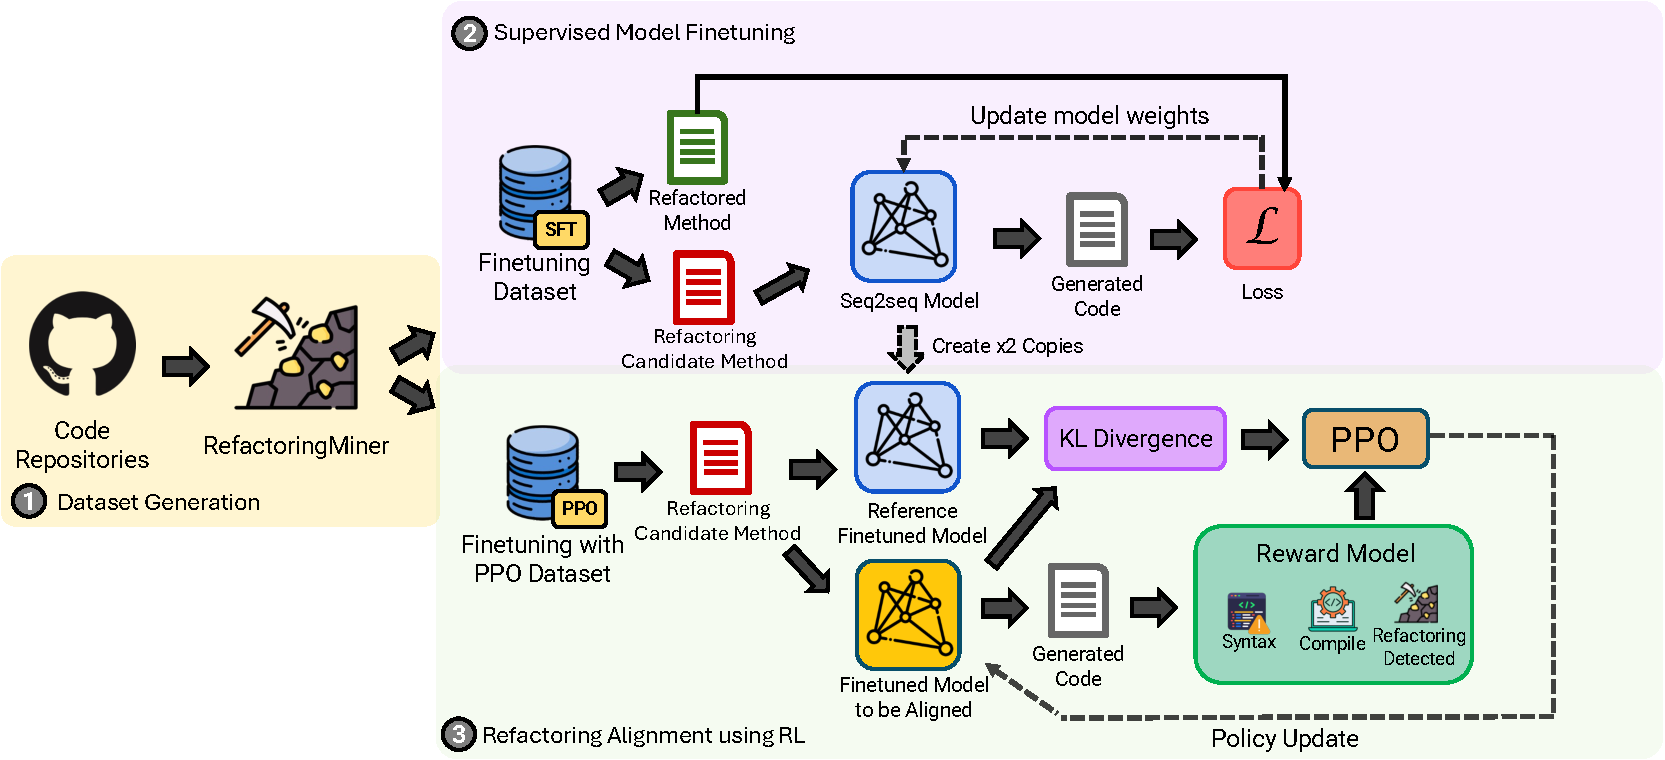
\includegraphics[width=\textwidth]{chapters/generation/images/overview_cropped.pdf}}
\caption{Overview of the proposed approach.}
\label{fig:methodology}
% \vspace{-5pt}
\end{figure*}

\subsection{Overview}
% \todo{Please follow goal -> RQs -> approach}

The goal of this study is to evaluate the effectiveness of fine-tuned \llmsc{}s pretrained on code and develop a deep reinforcement learning-based approach for generating code for extract method refactoring. We seek to demonstrate the effectiveness of our approach not only quantitatively but also qualitatively.
% This study proposes an approach to fine-tune a \LLM{} (LLM) using deep reinforcement learning for automatically generating extracted methods and modified original methods after performing \exm{} refactoring. 
We formulate the following research questions.
\newpage
\begin{description}

    \item [\textbf{RQ1.}] \textit{How does supervised fine-tuning perform for extract method refactoring task?}


By answering this research question, we aim to evaluate how well does supervised fine-tuning a code \llm{} perform in automatically performing \exm{} refactoring.


    % \item [\textbf{RQ2.}] \textit{How accurately a reinforcement learning approach performs for automating \exm{} refactoring?}
    \item [\textbf{RQ2.}] \textit{How well does a reinforcement learning approach perform for automating extract method refactoring?}


% This research question aims to assess whether \llm{}s pre-trained on code can be \textbf{directly} aligned using a reinforcement learning technique to perform \exm{} refactoring task effectively.
This question examines whether code \llm{}s can be directly aligned using reinforcement learning techniques to effectively perform \exm{} refactoring.


    % \item [\textbf{RQ3.}] \textit{How accurately a reinforcement learning approach aligned with fine-tuned \llmsc{} for code performs for automating \exm{} refactoring?}
    \item [\textbf{RQ3.}] \textit{How does a reinforcement learning approach, combined with fine-tuned \llm{}s, perform for automating extract method refactoring?}

This question assesses the impact of combining Proximal Policy Optimization (\ppo{}) with custom reward signals on a fine-tuned model's performance in \exm{} refactoring tasks.
\end{description}

Figure~\ref{fig:methodology} illustrates our methodology. We create our dataset by using the tools such as SEART tool~\cite{seart2021data} and RefactoringMiner~\cite{Tsantalis:TSE:2020:RefactoringMiner2.0, Tsantalis:ICSE:2018:RefactoringMiner}.
Following dataset preparation, we fine-tune four different models: \codetf{} and \plbart{}, which are encoder-decoder models, and \codegpt{} and \codegen{}, which are decoder-only models. We evaluate the performance of these models using both quantitative and qualitative measures. After conducting both quantitative and qualitative evaluations, we align the pre-trained model directly using the Proximal Policy Optimization (\ppo{}) algorithm. Subsequently, we align the fine-tuned model using the same \ppo{} algorithm.
We systematically evaluate the applied approach using standard evaluation metrics. We also evaluate the models qualitatively using three key checks \ie{} syntactic validity, compilability, and the presence of the desired refactoring in the generated code.

\subsection{Dataset Creation} \label{section:dataset_creation}

We employ a systematic approach to identify and collect extract method refactoring instances across multiple open-source Java repositories. Step~\circled{1} in Figure~\ref{fig:methodology} shows an overview of the dataset preparation pipeline. 
We use SEART~\cite{seart2021data} tool to select a  list of repositories for analysis. 
SEART tool is a GitHub project sampling tool,
offering various commonly used filters (such as number of commits and stars).
We obtain a list of all non-forked Java repositories 
created between $2013$ and $2023$, that are active in $2024$, 
have at
least $100$ commits,
and minimum $50$ stars. 
We obtained a total of $1,618$ repositories
satisfying the criteria.

\begin{algorithm}[th!]
\caption{Procedure for Creating Dataset}
\label{algo:1}
\begin{algorithmic}[1]
    \State \textbf{Input:} List of repositories $R = \{r_1, r_2, \dots, r.
    _n\}$
    \State \textbf{Output:} JSONL file with keys ``Input'' and ``Output''
    
    \Procedure{CreateDataset}{$R$}
        \State $Data \gets \emptyset$ \Comment{Initialize the dataset as an empty set}
        \For{each repository $r_i \in R$}
            \State Retrieve branch details for $r_i$
            \State Fetch the list of commits for the given branch
            \For{each commit $c_j$ in the list of commits}
                \State Identify refactorings performed in $c_j$
                \If{extract method refactoring is detected}
                    \State Extract metadata associated with the refactoring
                    \State Extract the refactored method using the metadata
                    \State Checkout to the previous commit $c_{j-1}$
                    \State Extract the original method from $c_{j-1}$
                    \State Create output JSON object 
                    \State Append this JSON object to $Data$
                \EndIf
            \EndFor
        \EndFor
        \State Store $Data$ in a JSONL file
    \EndProcedure

\end{algorithmic}
\end{algorithm}



To iteratively process the list of repositories to prepare the dataset, we created a custom Command Line Interface (CLI) tool. 
Algorithm~\ref{algo:1} provides a pseudocode of the functionality of the tool. 
% \todo{explain Algo 1} 
For each repository, we retrieve branch details and fetch the commit history. We then iterate through each commit, identifying any extract method refactorings performed using RefactoringMiner~\cite{Tsantalis:ICSE:2018:RefactoringMiner, Tsantalis:TSE:2020:RefactoringMiner2.0}. When such a refactoring is detected, the algorithm extracts relevant metadata and the refactored method from the current commit $c_j$. It then checks out the previous commit, $c_{j-1}$ to extract the original, pre-refactored method. This pair of pre- and post-refactoring methods, along with associated metadata (such as file path, class content and start and end line of the methods), is packaged into a JSON object. These JSON objects are accumulated into an array, which is ultimately stored in a JSONL file format. This approach enables the creation of a comprehensive dataset ($\mathcal{D}$) that captures the before and after states of extract method refactorings across multiple repositories.

% We iterate through this repository list, 
% passing the repository name and branch details to our CLI tool. 
% With the help of RefactoringMiner, the tool extracts the methods involved in \exm{} refactoring along with the associated metadata and stores all identified samples in \texttt{jsonl} file as json objects. 

\begin{table}[ht]
    \centering
    \caption{Dataset statistics} \label{tab:dataset_stats}
    \resizebox{\columnwidth}{!}{
        \begin{tabular}{ccc|ccc}
            \toprule
            \multirow{2}{*}{Dataset} & \multicolumn{2}{c}{Before pre-processing} & \multicolumn{2}{c}{After pre-processing} \\
            \cmidrule(lr){2-5}
& \makecell[c]{Avg.\\ source token\\ length} &  \makecell[c]{Avg. \\ target token\\ length} &  \makecell[c]{Avg.\\ source token\\ length} &  \makecell[c]{Avg.\\ target token\\ length} & \\
            \cmidrule(lr){1-5}
\makecell[l]{$\mathcal{D}_{SFT}$}& 412.77 & 446.13 & 184.26 & 241.63\\ \addlinespace
\makecell[l]{$\mathcal{D}_{RL}$} & 410.60 & 449.09 & 187.62 & 242.13 \\ \addlinespace
% \makecell[l]{$\mathcal{D}$} & 411.68 & 447.69 & 185.94 & 241.88 \\ 
            \bottomrule
        \end{tabular}    
    }
\end{table}
\vspace*{\fill}
% We applied the aforementioned procedure to process both  repository sets.
% \todo{change the acronym, as discussed.}
For RQ1 and RQ2, we use the entire dataset.
For RQ3,
we divide the dataset into two mutually exclusive subsets one for supervised fine tuning and the other for the aligning the fine-tuned model with deep reinforcement learning.
We divide the dataset to maintain data integrity and avoid data leak while training  for RQ3.
We divide the repository list of $1,618$ repositories, collected from the SEART tool, in half. We applied the aforementioned procedure to process both sets of repositories. This resulted in $38,441$ samples for the supervised fine tuning ($\mathcal{D}_{SFT}$) and $9,313$ samples for deep reinforcement learning ($\mathcal{D}_{RL}$).
However, the resulting datasets contained samples that exceeded the context window (maximum input sequence length) of our selected fine-tuning models.
Among these models, \texttt{Code-T5} has the smallest context window of $512$ tokens, while others support up to $2,048$ tokens. To ensure compatibility across all models, we use $512$ as our maximum context length, eliminating any samples that surpassed this $512$-token threshold. After pre processing, $\mathcal{D}_{SFT}$ contains $26,949$ samples and $6,528$ samples in $\mathcal{D}_{RL}$. 
Table~\ref{tab:dataset_stats} presents the average token length distribution for both the datasets. Finally, each of the dataset is divided in $70:20:10$ ratio for training, testing and validation.

\subsection{Training Models}



\subsubsection{Fine tuning LLMs}

% \todo{IP: Setup information}
We employ the following criteria to select the models for fine-tuning.
The selected models must belong to encoder-decoder or decoder-only architecture.
We exclude encoder-only models, such as CodeBERT, from our study because the encoder-only models are not well-suited for sequence-to-sequence (seq2seq) generation tasks~\cite{wang2023codet5+}.
% \todo{state any other criterion; like size? common used or should not be too big? - DONE}  
Encoder-only model architectures like \textsc{bert} are designed to understand input sequences but lack the ability to generate new ones. They're optimized for tasks like classification or feature extraction, not for producing variable-length outputs required in seq2seq tasks. Without a decoder component and autoregressive generation capability, these models can't effectively perform tasks such as translation or text generation that require producing new sequences based on input.
We select the following models, two belonging to encoder-decoder and two to decoder-only architecture family,
based on the the above-mentioned criteria.

\begin{itemize}
    \item \textbf{Code-T5}: \codetf{}~\cite{wang2021codet5identifierawareunifiedpretrained} is a pre-trained encoder-decoder model that incorporates token type information from code and employs an identifier-aware pre-training objective to better utilize identifiers. \codetf{} offers a unified framework that supports both code understanding and generation tasks, enabling multi-task learning. 
    This model has been successfully applied to various code related tasks such as code summarization~\cite{al2023extending, gu2022assemble}, code translation~\cite{kusum2022unsupervised} and vulnerability detection~\cite{paul2023, hou2024largelanguagemodelssoftware}.

    \item \textbf{PLBART}: \plbart{}~\cite{ahmad2021} 
    % \todo{structure references as <Last name><year> format}
    is a pre-trained sequence-to-sequence model that can perform a wide range of program and language understanding and generation tasks. It is trained on a large dataset of Java and Python functions along with their associated natural language text using denoising autoencoding. 
    \plbart{} has been used in various software engineering applications especially in program repair task~\cite{paul2023, wu2023effective}

    \item \textbf{CodeGPT-adapt}: \codegpt{}~\cite{lu2021codexgluemachinelearningbenchmark} is a GPT-2-based decoder-only Transformer model for code completion, pre-trained on Python and Java code from CodeSearchNet datasets. It learns code structure and syntax through pre-training, enabling it to generate code automatically.
    It has been widely used for code generation tasks such as code completion~\cite{li2024ircoco, hou2024largelanguagemodelssoftware}.

    \item \textbf{CodeGen}: \codegen{}~\cite{nijkamp2022codegen} is a Transformer-based autoregressive language model trained on natural language and programming language datasets. It employs next-token prediction as its learning objective and has shown outstanding performance in program synthesis tasks~\cite{christopoulou2022pangu}.

\end{itemize}

Step~\circled{2} in Figure~\ref{fig:methodology} illustrates the \textsc{sft} strategy employed for extract method refactoring. To train the encoder-decoder models, the pre-refactored code is first tokenized to serve as the input sequence. After a forward pass through the model, output tokens are generated and decoded using the same tokenizer. The resulting method is then compared to the ground truth, which includes both the extracted method and the modified original method post-refactoring. The model weights are updated based on the cross-entropy loss computed between the predicted and ground truth methods.

For decoder-only models, the training process is similar, with the key difference being in the format of the input. In this case, the input sequence is formed by concatenating the pre-refactored code and the ground truth output, separated by a special \textsc{[SEP]} token. This format enables the model to learn from both the context of the original code and the desired output sequence in a single input representation.


\subsubsection{Aligning the models with RL}

In this study, we fine-tune and align the selected \llm{}s for \exm{} refactoring using \rl{} techniques (step~\circled{3}). 
We model the code transformation problem as a Markov Decision Process (MDP).
We define the \textit{state} as the set of all possible code representations and the state transition function as appending the chosen refactored token to the current sequence.

Algorithm~\ref{algo:2} describes the pseudocode for aligning the fine tuned language model for extract method refactoring task. The algorithm starts with an initial policy (decision-making strategy) and a value function (which estimates how good a particular state is). It then goes through multiple training iterations to improve these over time. In each iteration, we sample a batch of code snippets from our \rl{} dataset. For each snippet, \textit{i.e.} the pre-refactored method, we use the current policy to generate a sequence of refactoring actions. To assess the quality of the sequence generated at each training step, we compute a reward based on three factors: syntactic correctness, compilation success, and whether the action is recognized as a valid refactoring. 


% \subsubsection*{Reward Modelling}

% We employ a carefully designed reward model to guide the reinforcement learning process. 
The reward function plays a crucial role in evaluating the quality and correctness of the refactoring suggestions produced by the model.
Our reward function consists of three key components, each addressing a specific aspect of the refactoring process:

\begin{enumerate}
    \item \textit{Syntactic Correctness:} We assess the presence of errors in the refactored code.
    For this purpose, we check the presence of error nodes in the Abstract Syntax Tree (\abst{}) generated by \textit{tree-sitter} of the generated code.
    \begin{equation} \label{eq:syntax}
        R_{syntax} = 
        \begin{cases}
            +1 & \text{if no error nodes} \\
            -1 & \text{if error nodes present}
        \end{cases}
    \end{equation}

    \item \textit{Compilation Success:} We verify whether the refactored code compiles successfully. While the compiler automatically checks for syntactic issues, separating syntactic correctness from compilation success allows us to provide the \rl{} model with more granular feedback. This distinction is important because refactored code might be syntactically correct but still fail to compile due to semantic errors.
    \begin{equation} \label{eq:compile}
        R_{compile} = 
        \begin{cases}
            +1 & \text{if code compiles} \\
            0 & \text{if code fails to compile}
        \end{cases}
    \end{equation}

    \item \textit{Refactoring Detection:} We validate the presence of extract method refactoring in the generated code using RefactoringMiner.
    \begin{equation} \label{eq: detect}
        R_{detect} = 
        \begin{cases}
            +1 & \text{if detected by RefactoringMiner} \\
            -1 & \text{if not detected}
        \end{cases}
    \end{equation}
\end{enumerate}

The sum of these individual components gives us the total reward for a given refactoring suggestion.

\begin{equation}
    R_{total} = R_{syntax} + R_{compile} + R_{detect}
\end{equation}

This reward function encourages the language model to generate syntactically correct, compilable code that successfully implements the extract method refactoring. 


The value head is used to estimate the value of the current state using the value function as shown in Equation~\ref{eq:value_func}. The algorithm then calculates how much better or worse each action was than expected (the \textit{advantage}). This information is used to update the policy, aiming to increase the probability of actions that led to high rewards. However, to ensure stable learning, the algorithm checks how much the new policy differs from the old one using a measure called KL divergence as described in equation~\ref{eq:kl_div}. If the difference is too large, the update is adjusted to prevent drastic changes. Finally, the value function is updated to better predict future rewards. By repeating this process many times, the algorithm gradually improves its ability to make good refactoring decisions. 


\begin{algorithm}
\caption{DRL Training for Extract Method Refactoring with KL Divergence}
\label{algo:2}
\begin{algorithmic}[1]
\Require Initial policy $\pi_\theta$, value function $V_\phi$, KL divergence coefficient $\beta$, weights $w_1, w_2, w_3$
\For{each training iteration}
\State Sample batch of code snippets from dataset
\For{each code snippet $x$}
\State Generate a refactored code snippet using current policy $\pi_\theta$
\State Compute syntactic correctness: $R_{syntax}$ using Eq.~\ref{eq:syntax}
\State Compute compilation success: $R_{compile}$ using Eq.~\ref{eq:compile}
\State Compute refactoring validity: $R_{detect}$ using Eq.~\ref{eq: detect}

\State Compute total reward: $R_{total} = w_1 \cdot R_{syntax} + w_2 \cdot R_{compile} + w_3 \cdot R_{detect}$
\State Estimate the value of the current state: $V_\phi(s)$
\State Calculate advantage: $A = R_{total} - V_\phi(s)$
\EndFor
\State Compute policy update to maximize:
\State \quad $J(\theta) = \mathbb{E}\left[\frac{\pi_{\theta}(a|s)}{\pi_{\theta_{old}}(a|s)} A\right] - \beta \cdot \text{KL}(\pi_{\theta_{old}} || \pi_{\theta})$
\State Apply the update to the policy: $\theta_{old} \leftarrow \theta$
\State Update value function to minimize: $L(\phi) = \sum (R_{total} - V_\phi(s))^2$
\EndFor
\end{algorithmic}
\end{algorithm}


\subsubsection{Fine tuning setup.} 

We fine-tune the supervised model for $10$ epochs on the dataset $\mathcal{D}$ for \textit{RQ1}, and on the dataset $\mathcal{D}_{SFT}$ 
for \textit{RQ3}. The training is conducted with a global batch size of $16$, using the Adam optimizer~\cite{kingma2017} with an initial learning rate of $1.33 \times 10^{-5}$. For aligning the models with \rl{}, we utilize and extend the \textsc{trl} Python library, which is widely used for training transformer language models with reinforcement learning. The generation parameters are set with \textit{min\_tokens} as $-1$ and \textit{max\_tokens} as $512$. The training consists of $20,000$ steps, with the model undergoing $10$ \ppo{} optimization epochs for each step. The code processes one batch per training step, generating responses, calculating rewards, and optimizing the model using PPO. For each batch, multiple internal PPO optimization passes are performed before moving to the next batch. This process repeats for $20,000$ steps, cycling through the dataset if necessary. A global batch size of $16$ is maintained, and the Adam optimizer~\cite{kingma2017} is employed. We apply Adaptive KL control with an initial KL coefficient of $0.2$. All experiments are conducted with a fixed seed value to ensure reproducibility and are performed on nodes of a High Performance Computing (HPC) cluster, utilizing $2$ V100-32GB GPUs and $32$ GB of RAM.

\subsection{Evaluation}
In this section, we summarize the metrics commonly used for code generation tasks.
Also, we provide details about qualitative evaluation that goes beyond the standard metrics.

\subsubsection{Evaluation Metrics}

To assess the effectiveness of our models quantitatively, we utilize established metrics from natural language processing field \bleu{}~\cite{papineni2002bleu} and \rouge{}~\cite{lin2004rouge}, as well as specialized metrics tailored for code evaluation, \codebleu{}~\cite{ren2020codebleumethodautomaticevaluation} and syntax match score~\cite{zhu2022xlcostbenchmarkdatasetcrosslingual}. 
The widespread adoption of these metrics in academic research for evaluating generative models supports our decision to use them. 


\subsubsection{Qualitative Evaluation} \label{subsubsection:qualitative}


To evaluate the effectiveness of our fine-tuned code language models in performing \exm{} refactoring, we construct a diverse test suite encompassing various 
complexity levels to ensure a thorough evaluation of the model's refactoring capabilities. To create the test cases for evaluation, we first identified pre-refactored original methods from the test sets of each of the dataset as mentioned in Section~\ref{section:dataset_creation}. We then selected 150 methods at random from $4,001$ test split samples ($2,695$ for \textsc{sft} and $1,306$ for \rl{}). Among these methods, few were very trivial like one or two liners and we discarded such methods. Finally, we collected $122$ such methods which underwent extract method refactoring across various repositories. 

A significant challenge in creating unit test cases is the lack of corresponding unit tests for many methods in the selected repositories.
To address this, we leveraged gpt-$4$o (version: gpt-4o-2024-05-13) API~\footnote{\href{https://platform.openai.com/docs/models/gpt-4o}{https://platform.openai.com/docs/models/gpt-4o}}
to generate unit tests and corresponding data. This approach aligns with recent research demonstrating the promising results of using language models for test case generation~\cite{tufano2020unit, nashid2023retrieval}. We specifically employed the \texttt{ChatTester} framework proposed by Yuan \etal{}~\cite{yuan2024chatgpt}, to generate unit tests for our samples. The framework utilized the class context of the smelly method, extracted as per Algorithm \ref{algo:1}, to create relevant unit test cases. The authors manually validated these generated test cases to ensure their quality and relevance. 
All the qualitative samples and corresponding test cases can be found in our replication package.

This combination of qualitative testing and quantitative analysis provides a systematic and objective assessment of our model's performance in extract method refactoring tasks. The multi-faceted evaluation approach allows for a comprehensive understanding of the model's capabilities and limitations across various \exm{} refactoring scenarios.


\section{Results}
% \section{Results}

\noindent
\subsection{RQ1: Performance of supervised fine-tuning for refactoring}

The research question aims to evaluate the performance of the fine-tuned models
for the refactored code generation.
The first part of Table~\ref{tab:all_metrics}
(\ie{} \textsc{pt + sft} column)
presents the results obtained by the considered models for the refactored code generation task. 
The results presented in the table demonstrate that the \plbart{} model outperforms other models metrics and code-specific evaluation measures. Specifically, \plbart{} achieves the highest scores on the \bleu{} and \rouge{} metrics, which assess the lexical and semantic similarity of the generated text to the ground truth. Crucially, \plbart{} also exhibits superior performance on the \codebleu{} metric, which captures the syntactic and structural fidelity of the generated code snippets.

\begin{table}[ht!]
    \centering
    \caption{Experimental results for different learning objectives. Here, PT, SFT, and RL refer to pre-trained, supervised fine-tuned, and reinforcement learning-based models}
    \resizebox{\columnwidth}{!}{
        \begin{tabular}{cccc|ccc|ccc}
        \toprule
        \multirow{2}{*}{Models} & \multicolumn{3}{c}{PT + SFT (RQ1)} & \multicolumn{3}{c}{PT + RL (RQ2)} & \multicolumn{3}{c}{PT + SFT + RL (RQ3)} \\
        \cmidrule(lr){2-4}
        \cmidrule(lr){5-7}
        \cmidrule(lr){8-10}
        & \makecell[c]{BLEU} & \makecell[c]{ROUGE} &\makecell[c]{CodeBLEU} & \makecell[c]{BLEU} & \makecell[c]{ROUGE} &\makecell[c]{CodeBLEU} & \makecell[c]{BLEU} & \makecell[c]{ROUGE} &\makecell[c]{CodeBLEU} \\
        \midrule
        \makecell[l]{Code-T5} & \makecell[c]{$67.80$} & \makecell[c]{$77.49$} &\makecell[c]{$53.13$} & \makecell[c]{$38.80$} & \makecell[c]{$37.62$} & \makecell[c]{$31.99$} & \makecell[c]{$\textbf{$75.91$\textsuperscript{$\bigstar$}}$} & \makecell[c]{$\textbf{$79.92$\textsuperscript{$\bigstar$}}$} & \makecell[c]{$\textbf{$61.87$\textsuperscript{$\bigstar$}}$} \\ \addlinespace
        \makecell[l]{PLBART} & \makecell[c]{$\textbf{68.28}$} & \makecell[c]{$\textbf{80.62}$} &\makecell[c]{$\textbf{55.66}$} & \makecell[c]{$30.21$} & \makecell[c]{$29.56$} & \makecell[c]{$22.48$} & \makecell[c]{$71.20$} & \makecell[c]{$69.68$} & \makecell[c]{$58.17$} \\ \addlinespace
        \makecell[l]{CodeGPT-adapt} & \makecell[c]{$62.68$} & \makecell[c]{$65.76$} &\makecell[c]{$49.29$} & \makecell[c]{$27.68$} & \makecell[c]{$30.76$} & \makecell[c]{$20.29$} & \makecell[c]{${64.96}$} & \makecell[c]{${67.82}$} & \makecell[c]{${47.99}$} \\ \addlinespace        
        \makecell[l]{CodeGen} & \makecell[c]{$59.32$} & \makecell[c]{$63.74$} &\makecell[c]{$42.11$} & \makecell[c]{$34.32$} & \makecell[c]{$33.74$} & \makecell[c]{$27.11$} & \makecell[c]{${61.59}$} & \makecell[c]{${60.52}$} & \makecell[c]{${46.67}$} \\
        \bottomrule
        
        \end{tabular}
    }
    
    \label{tab:all_metrics}
\end{table}

Furthermore, a comparative analysis reveals that \plbart{} substantially outperforms the \codetf{} model, achieving a $4.54\%$ higher \codebleu{} score. The performance gap is even more pronounced when contrasted with the \codegpt{} model, for which \plbart{} demonstrates an $12.98\%$ improvement on the \codebleu{} metric. These findings suggest that the \plbart{} model was successful in generating extract method refactored outputs that closely resemble the ground truth in terms of syntactic correctness.


To gain a more thorough understanding of the validity and robustness of the generated refactored outputs, additional validation checks and analyses are necessary. As detailed in Section~\ref{subsubsection:qualitative}, we
create a manually validated dataset for qualitative evaluation.
The dataset contains $122$ samples with before and after refactored code and corresponding test cases.
We use this qualitative dataset to check whether the trained model generates code without any syntactic and compilation errors, whether the generated code has extract method refactoring, and to what extent the generated code is passing the test cases.
Table~\ref{tab:exresults} presents the obtained results. 
For RQ1, notably, fine-tuned \codetf{} achieved the highest performance in qualitative evaluation. This supports our assertion that relying solely on quantitative metrics may yield misleading results and potentially produce low-quality refactored code.


\begin{boxH}
\textbf{RQ1 Summary:}
Fine tuning code \llm{}s show  an effective way to teach language models to generate refactored code automatically. Specifically, \plbart{} outperform other models in all the considered metrics. It show significant improvements over \codetf{} and \codegpt{}, particularly in \codebleu{} scores. 
% 74\% of \plbart{}'s outputs in the validation dataset exhibited desirable syntactic properties.
However, qualitative evaluation reveals that \codetf{} performs best in generating syntactically correct and functionally valid refactored code. 
% \todo{add qualitative results summary-DONE}
\end{boxH}


% \vspace{3mm}
\subsection{RQ2: Effectiveness of reinforcement learning for automated refactoring}

This research question aims to evaluate the application of \rl{} on the refactoring task when applied on pre-trained \llmsc{}.
The second part of the Table~\ref{tab:all_metrics} (\ie{} PT + RL column) shows
the obtained results.
Our results show that \codetf{} model demonstrates superior performance across all evaluation metrics compared to other language models when trained using \rl{}.

Interestingly, unlike the results observed in RQ1 with traditional fine-tuning, direct fine-tuning using \rl{} with Proximal Policy Optimization (\ppo{}) does not perform well.
% across all models. \todo{how did we know this? We dont have the results from the baseline (pure pre-trained models)
% But this is in comparison to the direct fine tuned models for which results are there in Table 2}
This outcome may be attributed to the complexity of the \exm{} refactoring task and the potential mismatch between the \rl{} objective and the nuanced requirements of code refactoring. Fine-tuning language models that have been pre-trained on tasks other than code refactoring directly using non-differentiable rewards poses challenges. The disparity between the pre-training task and the target task of code refactoring makes it difficult to effectively train the models using \rl{} techniques. 

\begin{table}[ht!]
\centering
\caption{Qualitative evaluation of fine tuned models}
\label{tab:exresults}
\rowcolors{2}{gray!25}{white}
\begin{tabular}{p{1cm}p{4cm}|%.5
>{\raggedleft\arraybackslash}p{2.5cm}%
>{\raggedleft\arraybackslash}p{2cm}%
>{\raggedleft\arraybackslash}p{2cm}%
>{\raggedleft\arraybackslash}p{2cm}%
>{\raggedleft\arraybackslash}p{2cm}%
}
&\textbf{Models} & \textbf{Syntactically correct (\%)}  & \textbf{Refactoring detected (\%)} & \textbf{Compile successfully (\%)} & \textbf{\# of unit tests passed (out of $122$)} \\ \midrule
&Code-T5 (FT) & $ \textbf{78.6} $  & $\textbf{66.4}$ & $\textbf{72.1}$ & $\textbf{41}$ \\
&PLBART (FT) & $76.9$ & $63.8$ & $69.5$ & $38$ \\
&CodeGPT-adapt (FT) & ${77.5}$ & ${64.3}$ & ${70.1}$ & $39$ \\
\multirow{-4}{*}{RQ1}&CodeGen (FT) & $78.3$ & ${65.1}$ & $71.2$ & $40$ \\ \midrule
&Code-T5 + RL & {21.4}  & {20.2} & {22.3} & {21} \\
&PLBART + RL & ${21.7}$ & ${18.9}$ & ${21.5}$ & ${16}$ \\
&CodeGPT-adapt + RL& ${19.7}$ & ${14.1}$ & ${20.2}$ & $14$ \\
\multirow{-4}{*}{RQ2}&CodeGen + RL & $23.6$ & ${19.2}$ & $21.1$ & $9$ \\ 
\midrule
&Code-T5 (FT) + RL & $\mathbf{85.7}$  & $\mathbf{74.9}$ & $\mathbf{79.8}$ & $\mathbf{66}$ \\
&PLBART  (FT) + RL & ${82.4}$ & ${71.6}$ & ${76.3}$ & ${58}$ \\
&CodeGPT-adapt  (FT) + RL& ${83.1}$ & ${72.2}$ & ${77.5}$ & $61$ \\
\multirow{-4}{*}{RQ3}&CodeGen  (FT) + RL & $84.3$ & ${73.5}$ & $78.6$ & $63$ \\ \bottomrule

\end{tabular}
\end{table}


Qualitatively also, as shown in \textit{RQ2} of Table~\ref{tab:exresults}, the generated refactorings exhibit poor quality. 

The \rl{} method's poor performance in functional areas highlights a misalignment with the refactored code's true requirements. This suggests that the \rl{} reward signals may insufficiently penalize syntactic and semantic errors, resulting in models 
% that excel in surface-level metrics but fail 
to produce functionally valid code. A potential explanation for this behavior could be that the \rl{}, performed on a generic pretrained language model, may not receive appropriate reward signals from our reward framework or the non-score rewards (KL divergence penalty). This hypothesis can be corroborated by examining Figure~\ref{fig:rl_stats}. Figure~\ref{fig:std_reward} illustrates the persistent high standard deviation of rewards for the \rl{} fine-tuned model throughout increasing training steps. This trend indicates that the reward signals fail to effectively steer the model towards optimal performance. Concurrently, Figure~\ref{fig:kl_penalty} reveals an upward trajectory in the KL-Divergence penalty over time. This escalation suggests a growing divergence between the trained model and the reference model, further supporting our hypothesis that the current reward system may be inadequate for guiding the model towards generating functionally sound code refactorings. 


\begin{boxH}
\textbf{RQ2 Summary:} Generating refactored code from a pre-trained model directly aligned with \rl{} does not produce comparable results to the corresponding fine-tuned models as shown in RQ1 quantitatively or qualitatively.

\end{boxH}





\subsection{RQ3: Evaluating the performance of reinforcement learning and fine-tuned LLMs for refactoring} 

In this research question, we aim to evaluate the efficacy of applying \rl{} to generate refactored code, focusing on model performance when fine-tuned using a combination of supervised fine-tuning (\textsc{sft}) and \rl{} objectives.
Specifically, we start with the trained fine-tuned models from RQ1, and train them with \ppo{} and reward from a feedback system to observe any improvements in the models compared to their fine-tuned counterparts.
% Our study investigated the efficacy of applying \rl{} to generate refactored code, focusing on model performance when fine-tuned using a combination of supervised fine-tuning (\textsc{SFT}) and \textsc{DRL} objectives. In RQ1, we examined the impact of maximizing the log-likelihood of the next correct code through \textsc{SFT}. RQ2 explored the effects of \textsc{DRL}, which aims to maximize the reward signal using a policy-based approach to select the optimal policy.

Table~\ref{tab:all_metrics} presents the results in the column titled PT + SFT + RL
along with results obtained in other settings as discussed in RQ1 and RQ2.
The results demonstrate that \textbf{the most effective outcomes are achieved when models are trained using both SFT and RL objectives.} This combined approach lead to significant improvements across various metrics. Specifically, we observed an approximate 10\% increase in \codebleu{} compared to models trained solely with \textsc{sft}, and an 11\% improvement over those trained exclusively with \rl{}. Similar performance gains were noted in other metrics, including \bleu{} and \rouge{}.
The superiority of the combined approach can be attributed to the complementary nature of \textsc{sft} and \textsc{rl}. \textsc{sft} excels at identifying inherent patterns and structures within data, primarily utilizing large labeled datasets. In contrast, \textsc{rl} adapts through environmental interactions, optimizing predefined reward metrics. By integrating these methodologies, our model can effectively navigate dynamic contexts while capturing underlying data patterns.

Our combined approach demonstrated a significant improvement in the evaluated quality metrics. The number of successfully passing test cases increased substantially, rising from $41$ in the best-performing model, \codetf{}, to $66$---a significant improvement of approximately $61\%$. Additionally, RefactoringMiner identified an increased number of cases, from $87$ to $98$. These results highlight the efficacy of \rl{} in producing accurate extract method refactored code.

Figure~\ref{fig:rl_stats} illustrates the trends in the standard deviation of rewards and the KL-Divergence penalty across training steps. The initial decline in standard deviation, followed by stabilization, coupled with consistent KL-divergence penalties, suggests that our reward modeling strategy effectively aligns a fine-tuned language model for the extract method refactoring task. These results collectively highlight the efficacy of \rl{} in producing accurate extract method refactored code.

\begin{figure*}[ht!]
    \centering
    \begin{subfigure}[t]{0.45\textwidth}
        \centering
        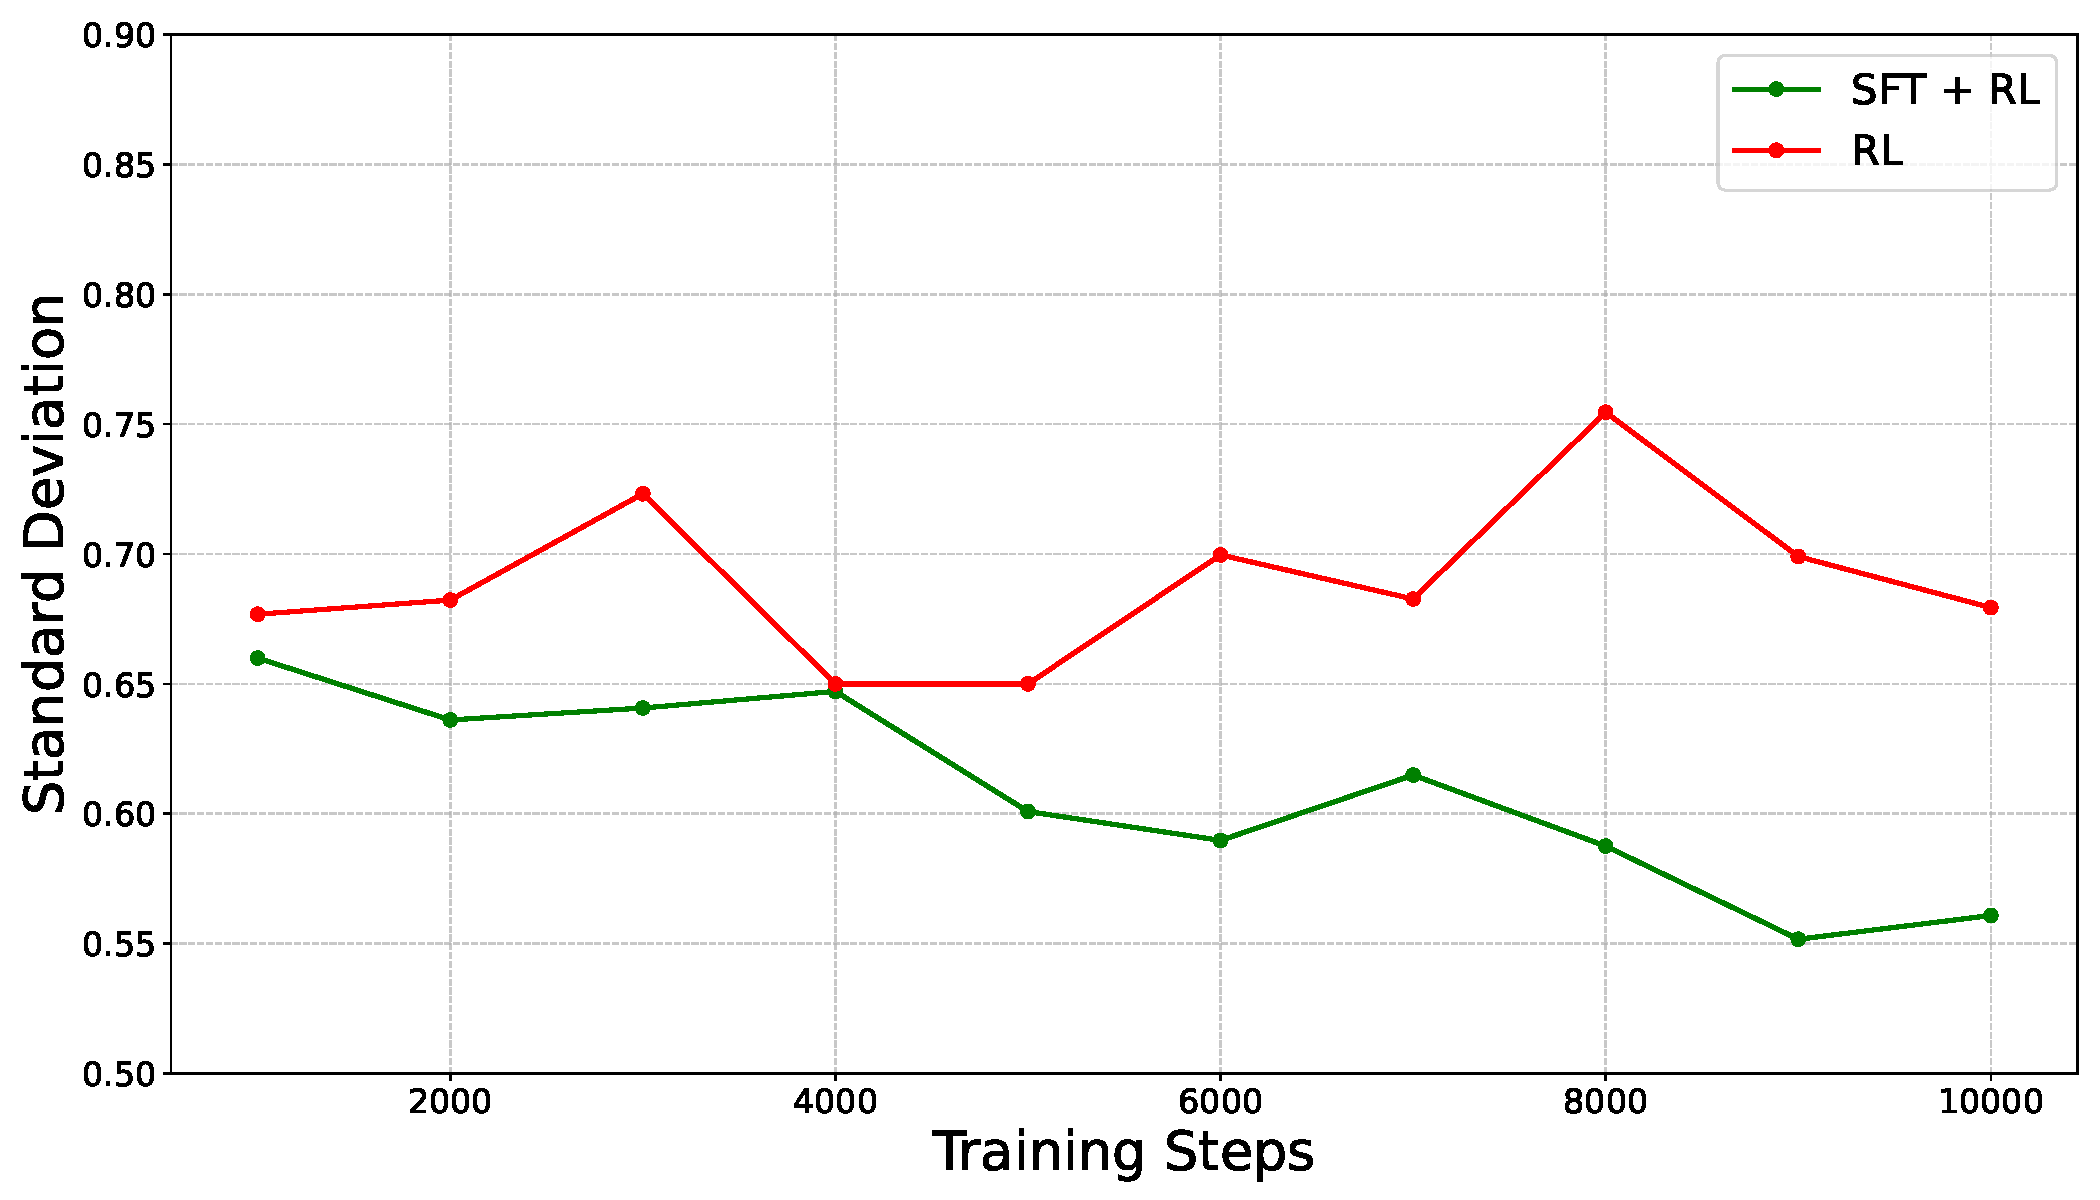
\includegraphics[height=1.5in]{chapters/generation/images/std_reward.pdf}
       \caption{Standard Deviation of Rewards}
        \label{fig:std_reward}
    \end{subfigure}
 ~
    \begin{subfigure}[t]{0.45\textwidth}
        \centering
        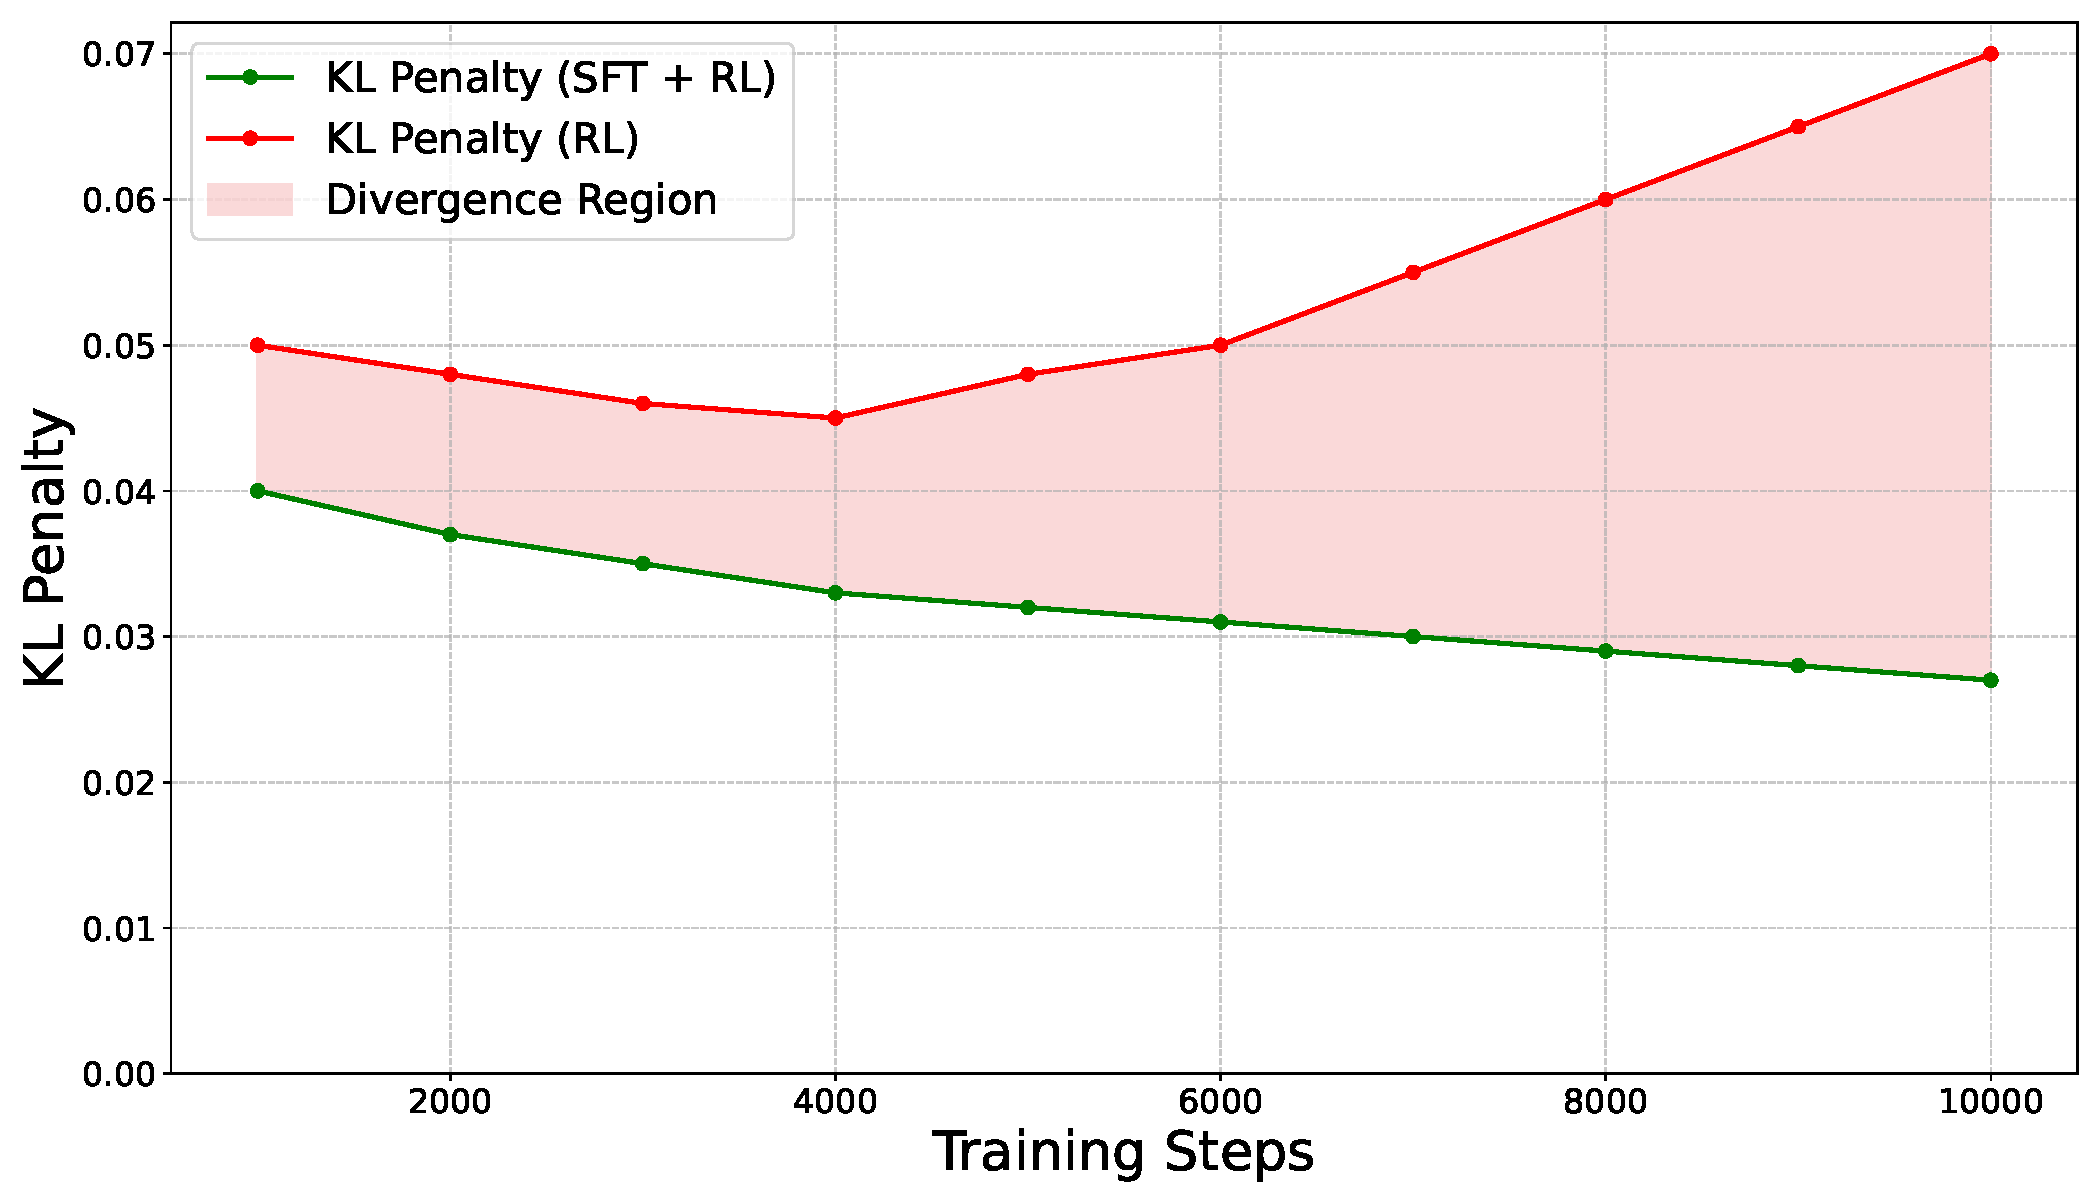
\includegraphics[height=1.5in]{chapters/generation/images/kl_penalty.pdf}
        \caption{Negated KL Divergence Penalty}
        \label{fig:kl_penalty}
    \end{subfigure}
    \caption{RL training observations}
    \label{fig:rl_stats}
\end{figure*}


While \textsc{sft} typically learns based on loss derived from labeled data, the integration with \textsc{rl} allows the model to benefit from a more comprehensive feedback system, including reward signals. This holistic approach contributes to the observed performance enhancements.

We present an illustrative example of a \exm{} refactoring in Figure~\ref{fig:example}, highlighting the differences of \sft{} and \rl{} techniques.
The original method belongs to \texttt{aws/aws-dynamodb-encryption\-java} repository as present in commit \texttt{ea43801}. 
Snippets \texttt{B} and \texttt{C} are generated by \sft{} model and combined \sft{} with \rl{} aligned models respectively. As we can see from the generated example, there are few syntactic errors (highlighted by red background color) present in the output generated by the fine-tuned only model. The combined \rl{} model seems to be more aligned to the ground truth. However, the generated code is not absolutely accurate because at line $10$ it throws an \texttt{IllegalArgumentException} instead of \texttt{IndexOutOfBoundException}. But this example strengthens our claims that the combined \sft{} model with \rl{} alignment enhances language model performance to generate more accurate extract method refactored code.

\begin{figure*}[ht!]
    \centering
    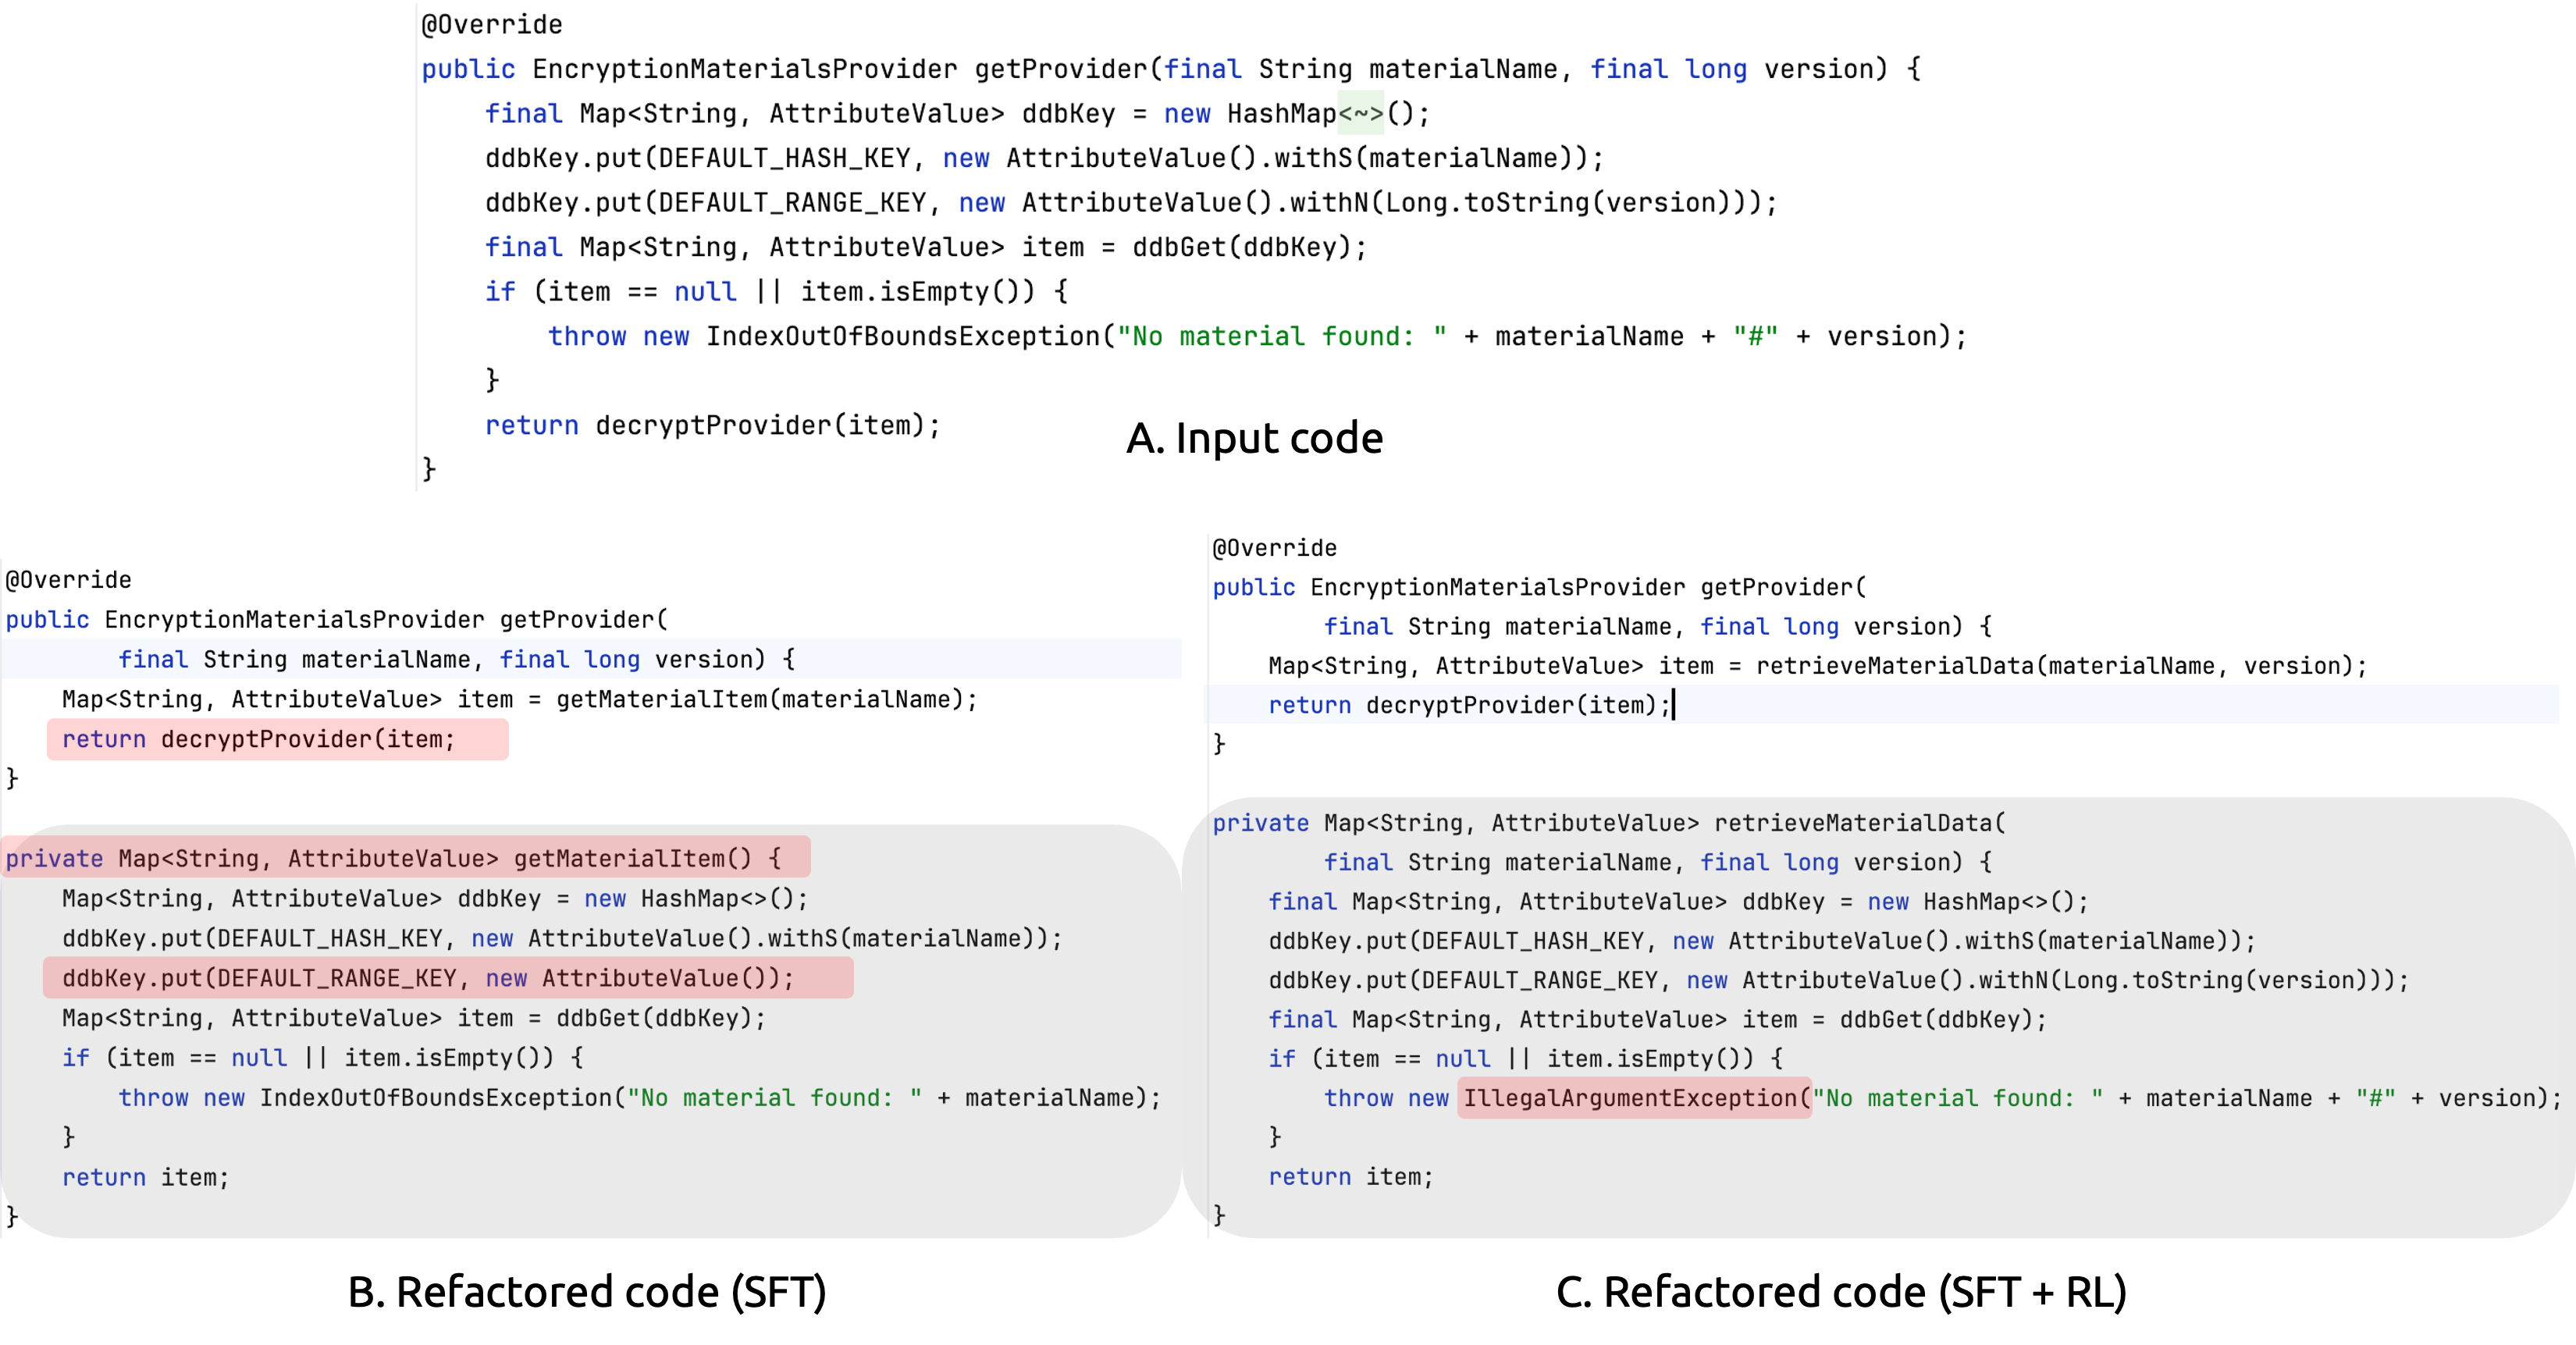
\includegraphics[width=\textwidth]{chapters/generation/images/example.png}
    \caption{Extract method refactoring example generated using Supervised Fine-Tuning (SFT) and the combination of SFT and Reinforcement Learning (RL) techniques}
    \label{fig:example}
\end{figure*}

\begin{boxH}
    \textbf{RQ3 Summary:} Our results demonstrates that combining supervised fine-tuning and \rl{} objectives yields superior results in generating refactored code. This integrated approach outperforms individual methods, showing significant improvements in \codebleu{}, \bleu{}, and \rouge{} metrics, while mitigating common limitations associated with single-objective training.
\end{boxH}


\section{Discussions}
While statistical metrics provide valuable insights, they may not fully capture a model's ability to generate high-quality code. 
We can observe the phenomenon in Table \ref{tab:all_metrics} and Table \ref{tab:exresults}.
The evaluation metrics used in Table \ref{tab:all_metrics} do not show very drastic difference in the RQ1 and RQ3 results.
However, the qualitative results presented in Table \ref{tab:exresults} present very different narrative.
We observe that the models trained using both supervised fine-tuning and \rl{} techniques show significantly better results. Specifically, the number of test cases passed by the best model in RQ3 is 61\% more than that of the best model in RQ1.
This observation highlights the importance of qualitative evaluation in addition to traditional metrics-based evaluation.


One may wonder whether production-ready \llmsc{} for code, such as GitHub Copilot, can achieve better performance in automated extract method refactoring. Although this is beyond the scope of our study, it's reasonable to assume that such models could handle smaller, frequently performed refactorings. However, anecdotal evidence suggests these models may struggle with context-specific, complex, non-atomic refactorings. Further research is needed to examine the behavior of these models across various prompt settings and complexity levels.

% \section{Related Work}
% 
% \todo{Add a section on usage of RL in SE - DONE}

\subsection{Automated Refactoring}

Many studies have explored automated refactoring candidate identification using machine learning techniques. Typically, these studies use source code metrics or commit messages to train models. Aniche \etal{}~\cite{Aniche2020Effectiveness} predict $20$ kinds of refactorings at method, class, or variable levels using code, process, and ownership metrics, with Random Forest performing best among six algorithms. Gerling~\cite{Gerling2020Machine} extended this work by improving the data collection process to create a high-quality, large-scale refactoring dataset. Van Der Leij \etal{}~\cite{van2021data} analyze five machine learning models to predict Extract Method refactoring, comparing results with industry experts. Using $61$ code metrics, they also found Random Forest to be the best performing model. Kumar \etal{}~\cite{Kumar2019Method} studied method-level refactoring prediction, analyzing 10 machine learning classifiers. Sagar \etal{}~\cite{Sagar2021Comparing} approaches refactoring candidate prediction as a multi-class classification problem, using both source code quality metrics and commit messages as features to predict six method-level refactorings. They compare text-based and source code-based models. Kurbatova \etal{}~\cite{Kurbatova2020Recommendation} employ code embeddings generated from Code2Vec~\cite{Alon2019Code2vec} to train their model for Move Method refactoring prediction.

In the domain of automated code refactoring, researchers have developed a variety of specialized tools and approaches. CeDAR~\cite{tairas2012cedar}, an Eclipse plugin, focuses on identifying and eliminating duplicate code. JDeodorant~\cite{JDeodrant, mazinanian2016jdeodorant} detects code smells and proposes refactoring strategies. Fokaefs~\etal{}\cite{fokaefs2012identification} extended JDeodorant's capabilities to prioritize and implement class extraction refactorings. SOMOMOTO\cite{zanetti2014automated} facilitates move method refactoring and code modularization. While these rule-based methods have made significant contributions, they face limitations in capturing semantic information during refactoring. Moreover, they often require manual intervention from developers to identify and select code blocks for refactoring. To address these challenges, recent research has explored the application of deep learning and large language models (LLMs) for automated code refactoring.

Szalontai~\etal{}~\cite{szalontai2023deep} developed a deep learning method for refactoring source code, initially designed for the Erlang programming language. Their approach comprises a localizer and a refactoring component, enabling the identification and transformation of non-idiomatic code patterns into idiomatic counterparts. Tufano~\etal{}~\cite{tufano2019learning} conducted a quantitative investigation into the potential of Neural Machine Translation (NMT) models for automatically applying code changes implemented during pull requests. Their approach leverages NMT to translate code components from their pre-pull request state to their post-pull request state, effectively simulating developer-implemented changes. To facilitate the rename refactoring process and reduce cognitive load on developers, Liu~\etal{}~\cite{liu2023refbert} proposed RefBERT, a two-stage pre-trained framework based on the BERT architecture. RefBERT is designed to automatically suggest meaningful variable names, addressing a challenging aspect of code refactoring.


Current automated refactoring tools lack semantic understanding and require manual intervention. To address this, we propose a hybrid approach combining supervised fine-tuning with reinforcement learning, enhancing the accuracy and completeness of extract method refactoring. This is the first study to apply deep reinforcement learning for this task, advancing automated refactoring tools.

\subsection{Reinforcement learning in software engineering}

Sequence modeling has emerged as a fundamental paradigm for addressing a wide array of software engineering challenges. In recent years, researchers have explored the application of deep reinforcement learning (DRL) techniques to mitigate exposure bias in supervised fine-tuned models for sequence generation tasks~\cite{ranzato2016sequenceleveltrainingrecurrent, keneshloo2019deepreinforcementlearningsequence}. Notably, Ranzato~\etal{}~\cite{ranzato2016sequenceleveltrainingrecurrent} pioneered the use of established metrics such as BLEU and ROUGE as reward signals in DRL algorithms to optimize network parameters in machine translation, effectively addressing exposure bias. The intersection of DRL and sequence modeling has led to innovative frameworks, such as the one proposed by Chen~\etal{}~\cite{chen2021decisiontransformerreinforcementlearning}, which reconceptualizes reinforcement learning problems as sequence modeling tasks. This approach has paved the way for novel applications in various domains.

In the realm of software engineering, DRL methods have gained traction, particularly in code completion and summarization tasks. Wang~\etal{}\cite{wang2022compilable} leveraged compiler feedback as a reward signal to enhance the quality of language model-generated code. Le\etal{}\cite{le2022coderl} introduced CodeRL, a framework that integrates RL with unit test signals to fine-tune program synthesis models. Shojaee~\etal{}~\cite{shojaee2023execution} conducted comprehensive research, proposing a framework for fine-tuning code language models using DRL and execution signals as rewards. Recent advancements in this field include IRCOCO by Li~\etal{}\cite{li2024ircoco}, which employs immediate rewards to fine-tune language models for code completion tasks. Wang\etal{}\cite{wang2024rlcoder} developed RLCoder, combining DRL with Retrieval-Augmented Generation (RAG) pipelines for repository-level code completion. Furthermore, Nichols\etal{}~\cite{nichols2024performance} demonstrated the potential of DRL in generating efficient parallel code, expanding the application of these techniques to performance optimization.

To our knowledge, \llm{}s have not been specifically trained or aligned for extract method refactoring. Our approach, which combines supervised fine-tuning with PPO alignment, is a first in this domain. This novel methodology produces accurate refactored methods, marking a significant advancement in the field.

\section{Threats to Validity}
% \section{Threats to Validity}
\noindent

\textit{\textbf{Internal validity:}} Internal validity concerns relate to the reliability of conclusions drawn from our experimental results. To enhance the trustworthiness of our findings, we implemented several measures. Firstly, we addressed the potential confounding effect of varying hyperparameters by utilizing consistent settings across all models, based on the optimal configurations identified in prior research by Li~\etal{}~\cite{li2024ircoco}. Additionally, we employed identical data splits for training and testing across all models, ensuring equal learning opportunities and evaluation conditions. These methodological decisions mitigate the risk of spurious results attributable to inconsistent experimental conditions, thereby strengthening the validity of our conclusions regarding the efficacy of deep reinforcement learning in generating refactored code methods.


\textit{\textbf{External validity:}} External validity concerns in our study pertain to the generalizability of our findings beyond the Java context. Despite this focus, we argue that our methodology is highly transferable. Our data collection technique is language-agnostic, applicable to any refactoring scenario. The general-purpose models we employed, trained on vast code corpora, are adaptable to various programming languages. While these factors suggest broad applicability, further research across multiple languages and environments would be necessary to conclusively establish the universal validity of our approach.


\chapter{Conclusions \& Future Work}
\epigraph{The best way to predict the future is to invent it.}{--- \textup{Alan Kay}}

\noindent

This thesis introduces a complete automated pipeline for extract method refactoring, encompassing both the identification of refactoring opportunities and their subsequent implementation. In this chapter, we summarize the results of our research, present the contributions of the thesis, elaborate our vision for future work, and conclude the thesis.

\section{Summary of the Results}

Automating software refactoring completely is an ambitious goal. To make meaningful progress in this direction, we focused our research on answering two fundamental questions. The first question addresses a common challenge developers face daily: identifying which code segments actually need refactoring. To tackle this challenge, we developed an innovative approach for identifying refactoring candidates. Our solution combines a self-supervised autoencoder with code representations from \GCB{}, a pre-trained language model, to capture the essence of source code. We then trained a binary classifier to identify potential extract method refactoring opportunities. The results were promising - our approach outperformed existing machine learning techniques by $30$\% in F1 score, demonstrating its effectiveness in identifying refactoring candidates.

Chapter 4 of this thesis presents our comprehensive solution that incorporates reinforcement learning to automatically perform extract method refactoring. We began by building a substantial dataset of real-world extract method refactoring examples from Java projects. Our evaluation covered various large language models, including both encoder-decoder and decoder-only architectures. An interesting finding emerged during our analysis - while \plbart{} showed strong performance in traditional metrics like \bleu{} and \rouge{}, its qualitative results fell short of expectations. This observation led us to develop an innovative hybrid approach that combines conventional fine-tuning with reinforcement learning alignment. This combination proved particularly effective, showing significant improvements across both quantitative and qualitative measures. The numbers tell a compelling story: our reinforcement learning-aligned approach improved upon traditional supervised fine-tuning by $11.96\%$ in BLEU scores and $16.45\%$ in \codebleu{} scores. Perhaps most importantly, we validated our approach through practical testing. When we ran our solution through a suite of $122$ unit tests, the reinforcement learning-aligned \codetf{} model successfully passed $66$ tests, compared to just $41$ for the baseline model. These results clearly demonstrate our approach's ability to generate not just syntactically correct, but functionally valid refactorings.

\section{Contributions of the Thesis}

The main contributions of this research can be summarized as follows:

\subsection{Research Contributions}

\begin{itemize}

\item We solved a fundamental problem in the field by creating a framework that can reliably tell apart good and bad candidates for \exm{} refactoring. Our experimental results showed significant improvement in accuracy than what was previously possible, making it much more practical for real-world use.

\item We developed a new way to understand code using Autoencoders with \GCB{}. This new approach proved better at capturing the subtle non-heuristics based patterns in code that make refactoring decisions more accurate.

\item By combining supervised learning with reinforcement learning, we created a hybrid system that's particularly good at automatically performing \exm{} refactoring. We observed significant performance improvement not only in terms of quantitative metrics but also validated our approach qualitatively using real world test cases. 


\end{itemize}

\subsection{Impact and Implications}
Our work has some exciting practical implications for software development:

\begin{itemize}
\item Developers can now save significant time on refactoring tasks both while identifying what to refactor and how to refactor with reduced chance of human error.

\item The high accuracy of our approaches and thorough validation of the generated results indicate that our solutions are ready for real-world use in development environments.

\item Since we've made everything open source, the developer community can build upon our work, adapt it to their needs, and keep improving it.

\end{itemize}

These advancements mean that developers can spend less time on routine code maintenance and more time on creative problem-solving. The tools we've developed aren't just theoretical - they're practical solutions that can make a real difference in day-to-day software development work.


\section{Future Work}

\subsection{Refactoring Candidate Identification}

For refactoring candidate identification, our future work will focus on exploring advanced architectural variations of embedding models that can better capture code semantics and structural patterns. As an extension of our current work, we look forward to perform an ablation study to better understand the impact of each of the components and how modifying them can affect the outcome. We plan to investigate hierarchical attention mechanisms and hybrid approaches that combine traditional software metrics with learned representations. This includes developing more sophisticated methods for handling context-dependent refactoring opportunities and exploring multi-modal learning approaches that can leverage both source code and documentation. 

\subsection{Refactored Code Generation}

In the domain of refactoring generation, we plan to enhance our reinforcement learning approach by developing more sophisticated reward functions that better capture code quality improvements and maintenance benefits. An in-depth analysis is required to better understand how the model performs in separating multiple concerns. We also plan to ensure the validity and reproducibility of our results by seeding and running the experiments multiple times. We aim to explore few-shot learning approaches that can adapt to project-specific coding standards and patterns, making the generated refactorings more contextually appropriate. Furthermore, we plan to make these techniques language and refactoring type agnostic.

\subsection{Integrating these solutions to production}

Looking ahead, our primary focus is to optimize the refactoring process for real-time performance, making it responsive enough to work alongside developers as they code. We aim to create a lightweight solution that maintains its high accuracy while integrating seamlessly with existing development environments. Beyond extract method refactoring, we plan to expand our approach to cover other important refactoring techniques. Our goal is to incorporate these capabilities into standard development workflows, making automated refactoring a natural and efficient part of the software development process.

This research lays the groundwork for more sophisticated automated code maintenance tools, opening new possibilities for improving software development practices.

\bibliographystyle{plain}
\bibliography{thesis}

\appendix

\chapter{Complementary Material}
This appendix presents the materials and tools used during this thesis.

\section{Replication Package}\label{appendix}

The framework, tools, scripts, analysis, and generated data can be found online at:

\begin{itemize}
    \item \href{https://github.com/SMART-Dal/extract-method-identification}{https://github.com/SMART-Dal/extract-method-identification}
    \item \href{https://anonymous.4open.science/r/extract-method-generation-2C9B}{https://anonymous.4open.science/r/extract-method-generation-2C9B}
\end{itemize}



\chapter{Copyright Release}
\section{Automatic refactoring candidate identification leveraging effective code representation}\label{copyright}

Palit, Indranil, Gautam Shetty, Hera Arif, and Tushar Sharma.“Automatic
refactoring candidate identification leveraging effective code representation.” In
2023 IEEE International Conference on Software Maintenance and Evolution
(ICSME), pp. 369-374. IEEE, 2023

Following is the copyright agreement with Institute of Electrical and Electronics
Engineers.

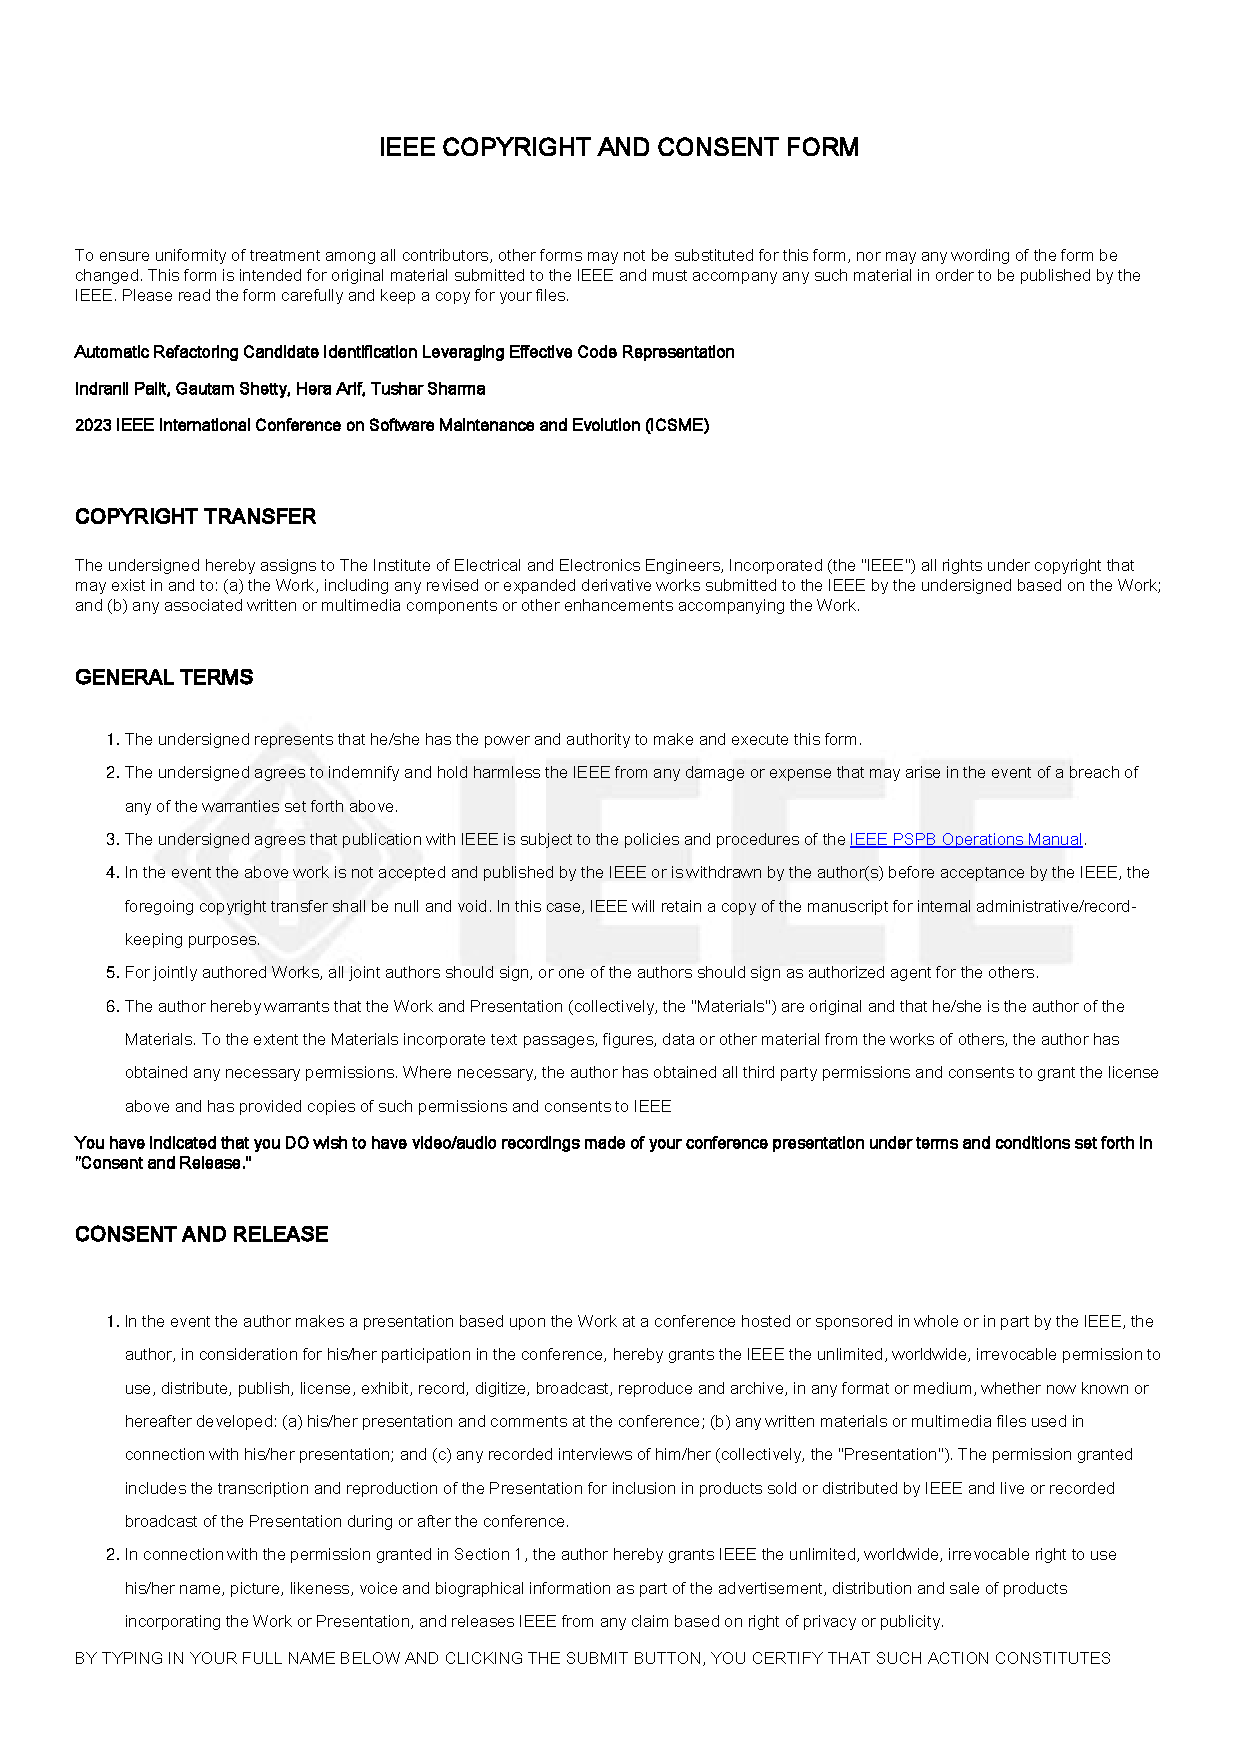
\includepdf[pages=-]{chapters/appendix/CopyrightReceipt.pdf}




\end{document}
